\documentclass[epsf,12pt,titlepage]{article}
\usepackage{epsfig}
\usepackage{amsmath}
\usepackage{fullpage}
\usepackage{makeidx}

\newcommand{\sub}[1]{\ensuremath{_{\mbox{\scriptsize \,#1}}}}
\newcommand{\supers}[1]{\ensuremath{^{\mbox{\scriptsize #1}}}}
\def\KT {\mbox{$k\sub{T}$} }
\def\epspace {$\eta$\,-$\varphi$ space }

\newcommand{\cname}[1]{\index{#1}\textsf{#1}}

\makeindex
\renewcommand\indexname{Functions and Classes}

\newenvironment{thinlist} {
    \begin{list} {---} {
        \setlength{\topsep}{0.075cm}
        \setlength{\parsep}{0.075cm}
        \setlength{\itemsep}{0.075cm}
    }
} {\end{list}}

\begin{document}

\title{FFTJet: The User Manual}

\author{Igor Volobouev, \ \ \ {\it i.volobouev@ttu.edu}}
% \date{Version: 1.5.0 \hspace{1.5cm} Date: \today}
\date{Version: 1.5.0 \hspace{1.5cm} Date: May 5, 2014}
\maketitle

\tableofcontents

\newpage
\section{Introduction}

\subsection{Intended Use}

The primary intended use of the FFTJet package is reconstruction of
particle jets in High Energy Physics collider data. FFTJet library allows the
user to implement a variety of jet reconstruction scenarios following
the same basic two-stage approach: first, pattern recognition is
performed whereby ``preclusters'' are found in the
      \epspace$\!\!$\footnote{The precise
      meaning of the $\eta$ variable
      is up to the user of the package
      (typically, this will be rapidity or pseudorapidity), while $\varphi$ is assumed
      to be the azimuthal angle of
      the energy deposit. Section~\ref{sec:discretization}
      provides more details.}
and then jets are reconstructed using preclusters as initial approximate
jet locations. This approach has several
important advantages over the cone, {\mbox{$k\sub{T}$}}, and anti-\KT jet reconstruction
algorithms commonly used at hadron collider experiments:
\begin{itemize}
\item The techniques used to determine the jet energies are not necessarily
      optimal for determining the event topology (the number of jets).
      These problems are distinct and should be solved separately.
\item FFTJet tools can be used to preserve as much
      energy flow information as possible within the jet reconstruction
      paradigm. This information is presented in a well-organized
      form convenient for pattern recognition applications and detailed
      analysis of jet substructure.
\item The computational complexity of the pattern recognition stage is
      $O(S N \log N)$, where $N$ is on the order of the number of towers
      in the detector calorimeter, and $S$ is the user-selectable
      number of resolution scales (cone and sequential recombination
      algorithms in their standard form use only
      one resolution scale). This complexity is independent from the
      detector occupancy and thus allows for predictable execution
      times which can be important for online use.
\item The main computational engine behind the pattern recognition
      stage is Discrete Fast Fourier Transform (DFFT). Due to widespread
      availability of DFFT implementations, the
      calculations can be performed on a variety of hardware including
      Digital Signal Processors (DSPs) and Graphics Processing Units (GPUs).
\item Reconstructed jets normally have well-defined shapes which simplifies
      energy calibration and pile-up subtraction.
\item The knowledge of the jet shape asymmetry in the \epspace can
      be effectively utilized which results in a superior algorithm
      performance in the presence of magnetic field.
\item The pattern recognition stage permits an efficiency
      correction which takes into account the detector boundary.
\item Provisions are made for efficient suppression of the detector noise
      both at
      the pattern recognition and at the energy reconstruction stages.
\end{itemize}
The jet energy reconstruction (a.k.a. recombination) stage which follows
pattern recognition supports both ``crisp'' and ``fuzzy'' clustering.
In the ``crisp'' clustering approach, each
calorimeter tower is assigned to a~single jet
(or to the underlying event/noise), just as in the \KT or cone algorithm.
In the ``fuzzy'' clustering each calorimeter tower
is assigned to every jet with a weight. Fuzzy clustering allows for modeling
such effects as the irreducible spatial energy smearing which occurs during
shower development inside particle calorimeters. 


\subsection{Emphasis on Pattern Recognition}

The jet reconstruction model implemented by the FFTJet package
was inspired by Refs.~\cite{ref:cheng} and~\cite{ref:modetree}
and initially proposed in~\cite{ref:igv2006}.
Ref.~\cite{ref:cheng} establishes an important connection
between the iterative cone algorithm (known as the ``Mean Shift''
algorithm in the pattern recognition literature) and
another statistical technique, kernel density estimation
(KDE)~\cite{ref:kde}. It turns out that
the locations of the stable cone centers correspond to
modes (peaks) of the energy
density built in the \epspace using kernel density
estimation with the Epanechnikov kernel. That is, all
such centers can be found by convolving the empirical energy density
$$
\rho\sub{emp}(\eta, \varphi) = \sum_{i} \varepsilon_{i} \delta^{2} (\eta - \eta_{i}, \varphi - \varphi_{i})
$$
with the function
$$
\mbox{Epanechnikov}(\eta, \varphi) = \left\{ \begin{array}{ll}
                           1 - (\varphi^2 + \eta^2)/R^2, & \varphi^2 + \eta^2 < R^2\\
                           0, & \varphi^2 + \eta^2 \ge R^2
                           \end{array}
                       \right.
$$
and then funding all local maxima of the convolution\footnote{The reader
familiar with the concept of ``Snowmass potential'' will recognize 
that this potential reproduces such
a~convolution up to a negative constant factor.}.
Here, $\varepsilon$ is an energy
variable whose actual meaning is user-defined (typically, transverse momentum
or transverse energy of a~particle, calorimeter tower, {\it etc.}) and $R$
is the cone radius in the \epspace$\!\!$.

The connection between the
iterative cone algorithm and KDE immediately suggests 
an~efficient implementation of a seedless cone algorithm: one should
discretize the calorimeter signals (or MC particles) on a regular
grid in the \epspace\!\!, perform the convolution
by DFFT, and find the peaks. This approach, however, does not
address an important problem inherent in the cone-based jet
reconstruction. This problem manifests itself as the pattern recognition
ambiguity illustrated in Figure~\ref{split}.
\begin{figure}[h]
\begin{center}
\leavevmode
\epsfxsize=2.5in
\epsfbox{split.eps}
\caption{The locations of the three stable clusters reconstructed by the ideal
iterative cone algorithm from two energy deposits are shown by the arrows
at the bottom.}
\label{split}
\end{center}
\end{figure}
Two energy deposits of similar magnitude
separated by a distance larger than $R$ but
smaller than $2 R$ produce three stable cone centers whose positions
are shown with the arrows at the bottom of the figure. In all current
implementations of cone-based jet reconstruction procedures, this
problem is addressed by the ``split-merge'' stage which happens after the
stable cone locations are determined. During this stage,
jets are merged if the energy which falls into the common region
exceeds a~predefined fraction of the energy of the jet with
smaller magnitude. Even if the search for stable
cones is performed in the infrared and collinear safe manner, the
outcome of the split-merge stage is no longer safe
because the decision on whether to merge two jets depends on the
minute details of the energy deposition structure.

Another way to look at this problem and a possible solution is illustrated
in Figure~\ref{trouble}.
\begin{figure}[t]
\begin{center}
\leavevmode
\epsfxsize=6.5in
\epsfbox{trouble.ps}
\caption{The convolution of two energy deposits with the Epanechnikov kernel (left)
and with two Gaussian kernels of different width.}
\label{trouble}
\end{center}
\end{figure}
The third stable cone center between the two energy
deposits happens because the sum of two Epanechnikov kernels placed
at the locations of the deposits has a spurious peak in the middle. However,
there is a variety of kernels which do not suffer from this problem.
In particular, the Gaussian kernel produces either two (narrow kernel) or one
(wide kernel) peaks, as shown. Even though
one still has to address the question
of choosing the kernel width, the Gaussian kernel has
a very important advantage: the whole split-merge stage is no
longer necessary.

An intelligent choice of the kernel width (or the $R$ parameter in the \KT
and cone algorithms) can not be performed until
some assumptions are made about the expected jet shapes. In fact,
optimal choice will be different for different signals. For example,
a data analysis which searches for high energy dijet events with two well-separated
jets is likely to make very different assumptions about jets from a~data
analysis which looks for $t\bar{t}$ events in the all-hadronic, 6-jet mode.
Moreover, the optimal width is not necessarily the same for every jet
in an event, as low momentum jets tend to have wider angular profiles,
especially in the presence of magnetic field. Because of this, it is
interesting to look at the jet structure of an event using a variety of
kernel width (cone radii, {\it etc.}) choices. In the limit of continuous
kernel width we arrive to a description of event energy flow known
as ``mode tree'' in the nonparametric statistics literature or
``scale-space image representation'' in the computer vision theory.
The information contained in such a description permits a variety of
optimization strategies for jet reconstruction which will be discussed
in section~\ref{sec:strategies}.

The FFTJet approach differs significantly from the majority of
jet reconstruction algorithms in the following way: FFTJet 
code by itself does not decide how
particle jets look like. Instead, the package user
is supposed to define a~jet shape model, and the
code will efficiently search for jet-like structures in the event
energy flow
patterns. The rationale for this view of jet reconstruction comes
from the realization that, in practice, the instrumental effects
(nonlinear response and finite energy resolution of the
calorimeter, presence of the
magnetic field in the detector, material in front of
the calorimeter, pile-up, noise, 
{\it etc.}) must be taken into account,
and will almost surely dominate the systematic error
of any precision measurement based on jets.
Therefore, a unified definition of ``what is a jet'' 
can not be achieved across detector measurements
in a variety of particle processes and HEP experiments.

The jet shape models supported by FFTJet
can range from very simple ({\it e.g.}, local
energy maximum within a sliding window in the \epspace\!\!) to quite
sophisticated ({\it e.g.}, energy and flavor-dependent jet fragmentation
function for several detector observables). If their
agreement with observations is good, complex models will
result in better statistical precision of jet energy determination.
On the other hand, simpler approaches can be less sensitive
to model misspecifications and will usually require less computing time.


\section{The Algorithm}

The users of the FFTJet package are expected to reconstruct jets
using the following sequence of steps:
\begin{enumerate}
\item The event energy distribution is discretized using a grid in the
      \epspace$\!\!$.

\item The discretized energy distribution is convolved with a kernel function
      $K(\eta, \varphi, s)$,
      where $s$ is the resolution
      scale parameter which determines the width and,
      possibly, the shape of the kernel. Many standard kernel functions are
      included in the FFTJet package, and user-defined kernels can be
      seamlessly added as well. The convolution is performed by DFFT.

\item The peaks of the convoluted energy distributions are found. These
      are potential ``preclusters''.

\item Preclusters with small magnitudes are eliminated in order
      to suppress the calorimeter~noise\footnote{Even in the
      absence of such noise, fake preclusters will be detected due to
      the presence of round-off errors in the DFFT procedure.}.

\item The previous three steps are repeated as many times as necessary
      using different values of $s$. The resulting preclusters are
      arranged in the ``clustering tree'' structure.

\item Using the clustering tree information and assumptions about
      expected signal signature, a~decision is made about the event topology
      by choosing a set of preclusters. These preclusters are passed to
      the jet energy reconstruction stage.

\item Reconstruction of the jet energies is performed
      as follows. The event is viewed as a~collection of energy deposits
      characterized by their direction $(\eta, \varphi)$ and
      energy $\varepsilon$.
      Depending on the environment in which the code is used,
      these deposits can originate from
      detector calorimeter cells, reconstructed tracks,
      Monte Carlo particles, {\it etc.}
      A~cluster membership function
      $M_{i}(\eta - \eta_i, \varphi - \varphi_i, \varepsilon, s_i)$
      is associated with
      each precluster $i$ at angular coordinates
      $(\eta_i, \varphi_i)$ and scale $s_i$. There is also a~membership function
      for the unclustered energy/underlying event. 

      The cluster membership functions
      are evaluated for every energy deposit in the event.
      In the ``crisp'' clustering scenario, an energy deposit is assigned to the jet
      whose membership function for this deposit is the largest. In the ``fuzzy''
      scenario, the deposit is split between all jets with weights
      proportional to their respective membership function values
      (the sum of all weights is normalized to 1 to ensure energy conservation).
\end{enumerate}
This sequence should work well for a wide variety of HEP data analyses.
Yet, if necessary, the balance between the code speed and the precision
of jet energy determination can be shifted in either direction.
For example, to speed things
up, the pattern recognition can be performed at a~single
predefined scale $s_0$. Alternatively, to further improve the jet energy
resolution, an iterative jet energy determination procedure can be
added as a final step. In such a procedure,
the jet directions $(\eta_i, \varphi_i)$
and the membership function scales $s_i$ are
updated at each iteration using
reconstructed jets from the previous iteration until
some convergence criterion is satisfied.

The rest of this section explains how to execute this plan
using the facilities provided by the FFTJet package.


\subsection{Basic Choices}
\label{basicchoice}

A large fraction of the FFTJet package code is provided
in the form of C++ templates. This implementation allows for a
significant flexibility in configuring the jet reconstruction procedure.
However, this also means that several decisions 
about classes and types used inside the templates must be made by the user:
\begin{itemize}
\item Which library to use for DDFT? This choice will determine which
      real and complex types FFTJet will operate on. FFTJet code uses
      external DDFT libraries through an~abstract interface:
      the \cname{AbsFFTEngine} class. The following concrete implementations
      of this interface are provided with the package:

      \cname{FFTWDoubleEngine}: interface to the double precision version
                                of the FFTW library from www.fftw.org.

      \cname{FFTWFloatEngine}: interface to the single precision version
                                of the FFTW library.

      \cname{CUFFTFloatEngine}: interface to the single precision DFFT
                                implementation in the NVIDIA Compute Unified
                                Device Architecture (CUDA). This interface
                                allows you to run parts of the FFTJet pattern
                                recognition code on modern NVIDIA graphics
                                cards.

      The FFTJet package can be interfaced to any other DFFT library by
      writing a corresponding adapter class derived from \cname{AbsFFTEngine}.

      FFTJet users are advised to structure their code in such a way
      that its dependence on a particular DFFT library is minimized.
      Whenever possible, the user code should rely upon the
      ``AbsFFTEngine.hh'' header rather than on one of the concrete
      implementation headers.
      This will allow for future DFFT library replacements with 
      minimal code adjustment.

\item How to represent 4-vectors? The 4-vector class
      performance can significantly affect the speed of the
      jet energy reconstruction stage. To be compatible with
      FFTJet, the 4-vector class must possess at least the following minimal
      set of features:
      \begin{thinlist}
        \item There is a way to build a vector from its coordinates.
        \item There is a default constructor which creates a null vector.
        \item The copy constructor and the assignment operator are defined
              ({\it e.g.}, generated by the compiler).
        \item Binary multiplication operator is defined for multiplying
              a vector (on the left) by a double (on the right).
        \item Operator += is defined for in-place addition of one vector to another.
      \end{thinlist}
      Any class which is syntactically compatible with the above
      requirements can be used with the jet energy recombination
      algorithms provided by the FFTJet package. It is likely that
      such a class would already be available to the package user
      (``HepLorentzVector'' class from the CLHEP
      library~\cite{ref:clhep} is a typical example).
      Due to an extensive use of vector algebra by the FFTJet code, simple
      and efficient 4-vector implementations without virtual methods
      should be preferred. One such implementation can be found in the
      ``examples/kinematics'' subdirectory of the package
      (class \cname{rk::P4} declared in the header file ``rk.hh'').
\end{itemize}
It is convenient to summarize these decisions in a header file which
contains the relevant ``typedef'' statements. The ``fftjet\_typedefs.hh''
file in the ``examples'' subdirectory of the package illustrates this approach.


\subsection{Energy Discretization}
\label{sec:discretization}

The purpose of the energy discretization step
is to create a grid equidistant in the \epspace
and to populate this grid with the observed energy
values. The exact meaning of $\eta$ and ``energy'' is
up to the package user ---  the package itself does
not make any assumptions. Some reasonable convention should
be adopted. In the analysis of experimental data,
it is common to reconstruct jets using pseudorapidity
for $\eta$ and transverse energy for
``energy''\footnote{Using rapidity and transverse momentum instead, one arrives
at a procedure which is invariant under boosts along the beam direction.
This approach can be attractive for theoretical studies.
However, these quantities can not be determined
by realistic calorimeters which measure  energy and direction.}.
The $\varphi$ is assumed to be the azimuthal angle of
the energy deposit.

The grid in the \epspace is created
using the \cname{Grid2d} class. The class constructor
declaration looks like this:
\begin{verbatim}
Grid2d(unsigned nEtaBins, Real etaMin, Real etaMax,
       unsigned nPhiBins, Real phiBin0Edge,
       const char* title = "");
\end{verbatim}
The constructor arguments are as follows:
\vskip2mm

\noindent \begin{tabular}{ll}
nEtaBins & Number of cells in the $\eta$ direction. \\
etaMin, etaMax & The grid boundaries in $\eta$. \\
nPhiBins & Number of cells in $\varphi$. \\
phiBin0Edge & Azimuthal angle of the boundary separating $\varphi$ cells with numbers \\
            & 0 and nPhiBins$-$1. \\
title & An arbitrary name for the grid. Intended for subsequent use by \\
      & some user-developed code which visualizes the grid contents. \\
\end{tabular}

\vskip2mm
\noindent It is convenient to think that the grid splits the \epspace
into rectangular cells, like a~histogram. The cell with index $(i,j)$ has corners at
\begin{eqnarray*}
(\eta, \varphi)\sub{bottom,left} & = & (\mbox{etaMin} + i\, \frac{\mbox{etaMax} - \mbox{etaMin}}{\mbox{nEtaBins}}, \ \mbox{phiBin0Edge} + j\, \frac{2 \pi}{\mbox{nPhiBins}})\\
(\eta, \varphi)\sub{top,right} & = & (\mbox{etaMin} + (i+1) \frac{\mbox{etaMax} - \mbox{etaMin}}{\mbox{nEtaBins}}, \ \mbox{phiBin0Edge} + (j+1) \frac{2 \pi}{\mbox{nPhiBins}})
\end{eqnarray*}
where $0 \le i < \mbox{nEtaBins}$, $0 \le j < \mbox{nPhiBins}$.

The cell sizes in $\eta$ and $\varphi$ should be normally chosen
in such a way that they reflect the granularity of the calorimeter used to
measure the jet energy. Ideally, the cell width in $\varphi$ (which is just $2 \pi/$nPhiBins) should be equal to the
calorimeter segmentation in $\varphi$, and the cell width in $\eta$
should be equal to the finest calorimeter segmentation in $\eta$.
On the other hand, choice of ``nEtaBins'' and ``nPhiBins'' parameters
should allow for subsequent efficient DFFT of the grid data, so that
exact powers of two are preferred\footnote{The majority of DFFT libraries only
support transforms of certain sizes. Check with the DFFT library description
for details.}. The grid boundaries in $\eta$ should be chosen in such a way
that the grid $\eta$ range not only fully covers the $\eta$ acceptance
region of the calorimeter but also exceeds it by some reasonable
amount. This excess
is needed to provide a guard area against spill-overs from high $\eta$ into
lower $\eta$ region (and back) during convolutions\footnote{These spill-overs 
happen because 2d DFFT assumes periodical structure not just
in $\varphi$ but also in $\eta$; the effective topology
therefore becomes toroidal rather than cylindrical. For more details
see, {\it e.g.}, section 13.1 in Ref.~\cite{ref:numrecipes}.}.

In case the energy distribution does not have a natural granularity
(e.g., when Monte Carlo particles are clustered)
the size of the grid cells should be chosen in such a way that
the binning effects do not prevent you from seeing the smallest
resolution details you are interested in. A good rule of thumb
(based on the Nyquist sampling theorem) is that in each direction
the discretization
grid granularity
should be two times finer than the smallest
interesting detail.

\subsubsection{Filling the Grid}

It is assumed here that the same \cname{Grid2d} object is
used to analyze a large number of events.
The ``reset'' method should be used to clear the grid
between these events.
The grid is normally filled using either ``fillFast'' or ``fill''
methods. One of these methods should be called for every
energy deposit in the event. The signature is as follows:
\begin{verbatim}
void fillFast(Real eta, Real phi, Real energy);
void fill(Real eta, Real phi, Real energy);
\end{verbatim}

The ``fillFast'' method works just as you would expect a typical histogram
filling function to work: the index of the rectangular
cell within which eta and phi values fall is determined, and 
the energy of that cell is incremented by the given amount.
The ``fill'' method is somewhat different: it distributes
the energy between four nearest grid cells in such a way that the
energy centroid in the \epspace coincides with the direction provided by the
eta and phi arguments.

\subsubsection{Energy Discretization for Realistic Detectors}

The granularity of calorimeters in HEP experiments is usually not
constant throughout the full $\eta$ acceptance range. Even if the
locations and sizes of discretization grid cells match the calorimeter
tower locations fairly well in some $\eta$ region (e.g., in the
barrel not far from $\eta = 0$),
such matching can not be maintained everywhere. Moreover,
some experimental setups use hexagonal towers which can
not be easily matched to a rectangular grid.

Typically, the
signal location within a single calorimeter tower can not be
determined, and it becomes natural to assume a~flat probability
distribution for the signal location across the tower face.
To carry the information contained in
this assumption through the signal discretization
process, the user
of the FFTJet package is encouraged to create a table of weights
with which each calorimeter tower contributes to the nearby grid
cells. The signal observed in the tower should then be divided
among the cells in proportion to the weights.

The weights can be determined by calculating the amount of overlap
in the \epspace between the grid cell areas and the tower face.
This calculation can be performed by the functions \cname{rectangleRectangleOverlap}
and \cname{rectanglePolygonOverlap} declared in the ``rectangleOverlap.hh''
header. Please check this header for more details
about the usage of these functions.

If the user creates such a table of weights, the signal discretization
should be performed using either ``fillBin'' or ``uncheckedFillBin'' methods
of the \cname{Grid2d} class. The signature of these methods looks like this:
\begin{verbatim}
void fillBin(unsigned etaBin, unsigned phiBin, Real energy);
void uncheckedFillBin(unsigned etaBin, unsigned phiBin, Real energy);
\end{verbatim}
The ``uncheckedFillBin'' function works slightly faster
by not testing whether the ``etaBin'' and ``phiBin''
arguments are valid. The ``energy'' argument 
should be set to the transverse energy (transverse momentum, {\it etc.}) of the
calorimeter tower multiplied by the weight with which this tower contributes
to the grid cell with index (etaBin, phiBin).

\subsection{Finding the Preclusters}

The FFTJet package provides a high-level driver class
for finding the preclusters (steps 2 through 5 of the algorithm
sequence): \cname{ClusteringSequencer}.
The simplest way of performing the pattern recognition with
FFTJet consists in constructing an object of this class
at the beginning of the data analysis job and then running
its ``run'' function on each discretized event.
The most important part of the \cname{ClusteringSequencer} declaration
(in the ``ClusteringSequencer.hh'' header file) looks like this:
\begin{verbatim}
template<typename Real>
class ClusteringSequencer
{
public:
    ClusteringSequencer(
        AbsConvolverBase<Real>* convolver,
        Functor1<bool,Peak>* selector,
        const PeakFinder& peakFinder,
        const std::vector<double>& initialScales,
        unsigned maxAdaptiveScales=0, double minRatioLog=0.01);

    virtual int run(const Grid2d<Real>& eventData,
                    AbsClusteringTree<Peak,long>* outputTree);

    virtual int insertCompleteEvent(
             double scale, const Grid2d<Real>& eventData,
             AbsClusteringTree<Peak,long>* outputTree, double dataCutoff=0.0);
};
\end{verbatim}
As you can see, this driver class is a template. Its argument
type, ``Real'', must be compatible with the
DFFT library chosen. The constructor arguments have the
following meaning:
\vskip2mm

\noindent \begin{tabular}{ll}
convolver & A pointer to an object conforming to the \cname{AbsConvolverBase} interface.\\
& Such objects calculate and manage Fourier transforms of the data \\
& and the kernels and perform their convolutions.\\
selector & A pointer to an object conforming to the 
\cname{Functor1}$<$bool,Peak$>$  \\
& interface. Such objects are used to eliminate fake preclusters.\\
peakFinder & An object which finds the modes of the convolved energy distributions.\\
initialScales & A collection of resolution scales for which the peak finding will be \\
& performed.\\
maxAdaptiveScales & Maximum number of additional scales to use for adaptive pattern \\
& recognition.\\
minRatioLog & This parameter determines the minimum separation between the \\
& scales used in the adaptive pattern recognition stage.
\end{tabular}

\vskip2mm
\noindent The clustering sequencer will not own the \cname{AbsConvolverBase}
and \cname{Functor1}$<$bool,Peak$>$ objects, that is, it will not attempt
to call the ``delete'' operator on the ``convolver''
and ``selector'' pointers in its own destructor. It is a responsibility
of the user of this
class to make sure that the "run" method is called
only when the objects to which these pointers refer are still alive.
The ``run'' arguments are as follows:
\vskip2mm

\noindent \begin{tabular}{ll}
eventData & Discretized event energy distribution.\\
outputTree & A pointer to an object conforming to the \cname{AbsClusteringTree} interface. \\ & Such objects are used to arrange pattern recognition results in a form\\
& convenient for subsequent analysis.
\end{tabular}
\vskip2mm
\noindent After calling the ``run'' method, the user can also invoke
the ``insertCompleteEvent'' function. This function inserts the whole
event into the clustering tree at the lowest resolution scale.
It will be useful to perform this insertion if the clustering tree
is going to be utilized as a~balltree~\cite{ref:balltree}
during subsequent pattern recognition calculations.


\subsubsection{AbsConvolverBase and its Implementations}

Note that the kernel which is convolved with the event data during
the pattern recognition stage does not change from one event to another.
This means that the Fourier images of such a kernel can
be calculated only once for each scale and then stored
for subsequent lookups. The \cname{AbsConvolverBase}
class declares an interface to the relevant services for the rest
of the FFTJet package code.

Multiple concrete implementations of the \cname{AbsConvolverBase} functionality
are provided with the FFTJet package: \cname{KernelConvolver},  
\cname{FrequencyKernelConvolver},
\cname{MultiKernelConvolver}, \cname{SequentialConvolver},
and \cname{FrequencySequentialConvolver}. 
The \cname{KernelConvolver} class implements
a basic model in which the discretized event 
data is convolved with a~single kernel
$K(\eta, \varphi, s)$ whose
functional form in provided in the $\eta$\,-$\varphi$ space.
The \cname{FrequencyKernelConvolver} performs convolutions
with a~single kernel represented in the frequency domain.
The \cname{MultiKernelConvolver} convenience class allows
the user to construct sophisticated kernels by multiplying and/or
dividing images of simpler kernels in the frequency space
(which corresponds to their convolution and/or
deconvolution in the \epspace\!\!). \cname{SequentialConvolver} and
\cname{FrequencySequentialConvolver} perform sequential 1-d Fourier
transforms instead of 2-d transforms. This can be useful in case
expected jet shape is different for different $\eta$ bins\footnote{
For example, the effect of the magnetic field
on the jet shape observed in the detector
depends on the radial distance at which the jet hits the calorimeter.
This distance will be $\eta$-dependent for calorimeters placed at
the detector sides (wall, plug, endcap).}.

The user of the FFTJet package would normally only
need to know how to construct one of the concrete convolver classes,
while the remaining \cname{AbsConvolverBase} methods
are needed for internal package functionality and are not
of particular interest to the application developers.
The declaration of the simpler \cname{KernelConvolver} constructor
looks like this:
\begin{verbatim}
template<typename Real, typename Complex>
class KernelConvolver : public AbsKernelConvolver<Real, Complex>
{
public:
    KernelConvolver(const AbsFFTEngine<Real,Complex>* fftEngine,
                    const AbsKernel2d* kernel,
                    unsigned minFixBin=0, unsigned maxFixBin=0);
};
\end{verbatim}
The ``Real'' and ``Complex'' template parameters must be compatible with the
DFFT library chosen. For its operation, \cname{KernelConvolver}
needs instances of \cname{AbsFFTEngine} and \cname{AbsKernel2d}
classes. The former class has already been discussed in section~\ref{basicchoice},
while the latter represents the kernel function in the \epspace\!\!.
A variety
of such functions is supplied with the FFTJet package; the choice
of the kernel is discussed in more detail in section~\ref{sec:kernelchoice},
and the complete
list of kernels is provided in the Appendix~\ref{appKern}.
The arguments ``minFixBin''
and ``maxFixBin'' can be used to request a clustering efficiency correction
near the detector boundary. It is assumed that the energy discretization
grid $\eta$ bins with numbers equal to and above ``minFixBin'' but
below ``maxFixBin'' correspond to the detector fiducial region.
If either ``minFixBin'' or ``maxFixBin'' parameter has any
other value besides default~0, the \cname{KernelConvolver}
code will provide a clustering
efficiency correction by multiplying the grid data with an
$\eta$-dependent efficiency flattening curve which ensures
that the total energy between ``minFixBin'' and ``maxFixBin''
remains constant and does not depend on the kernel scale
(that is, energy leakage outside the given
$\eta$ range due to convolution is prevented). It is not clear at this
time how such a procedure affects the angular resolution of
the preclusters and subsequent jet reconstruction steps,
so this feature should be considered experimental.

The \cname{FrequencyKernelConvolver} constructor is very similar. The only
difference is that it takes a pointer to an instance of the
\cname{AbsFrequencyKernel} abstract class instead of \cname{AbsKernel2d}.
Classes derived from \cname{AbsFrequencyKernel} calculate two-dimensional
kernels directly in the frequency domain.

The \cname{MultiKernelConvolver} constructor is slightly more complicated:
\begin{verbatim}
template<typename Real, typename Complex>
class MultiKernelConvolver : public AbsKernelConvolver<Real, Complex>
{
public:
    MultiKernelConvolver(const AbsFFTEngine<Real,Complex>* fftEngine,
                         const KernelSet* kernelSequence,
                         unsigned minFixBin=0, unsigned maxFixBin=0);
};
\end{verbatim}
The meaning of the ``fftEngine'', ``minFixBin'', and ``maxFixBin''
parameters is the same as in the \cname{KernelConvolver} constructor.
The ``kernelSequence'' parameter is a pointer to a~collection of kernels
which are combined in the frequency space. The kernel image
is built by the \cname{MultiKernelConvolver} according to the following
formula:
\begin{equation}
\label{eq:multikernel}
F_K(\vec{\omega}, s) = \frac{\prod_i F_{A_i}(\vec{\omega}, s) \prod_i F_{B_i}(\vec{\omega}, s)}{\prod_i F_{C_i}(\vec{\omega}, s) \prod_i (1 + |F_{D_i}(\vec{\omega}, s)|^2)} 
\end{equation}
For every $i$, $A_i$ is a kernel whose
functional form in provided in the frequency space.
$B_i$ and $C_i$ are kernels whose
functional forms are provided in the $\eta$\,-$\varphi$ space.
$|F_{D_i}(\vec{\omega}, s)|^2$ is a~power spectrum
of a kernel $D_i$ whose
functional form in provided in the $\eta$\,-$\varphi$ space.
This form of the convoluted kernel image is sufficiently
general to allow for a variety of convolution/deconvolution
approaches to event reconstruction. 
The kernels $A_i$, $B_i$, $C_i$, and $D_i$ are specified using
the helper class \cname{KernelSet}:
\begin{verbatim}
class KernelSet
{
public:
    explicit KernelSet(bool ownsPointers,
                       double regularizationFraction=0.0);

    void setRegularizationFraction(double fraction);

    std::vector<const AbsFrequencyKernel*> filter;
    std::vector<const AbsKernel2d*> numerator;
    std::vector<const AbsKernel2d*> denominator;
    std::vector<const AbsKernel2d*> denoiser;
};
\end{verbatim}
The correspondence between the class members and the Eq.~\ref{eq:multikernel}
components is realized as follows:

$A_i$ --- \verb[filter[

$B_i$ --- \verb[numerator[

$C_i$ --- \verb[denominator[

$D_i$ --- \verb[denoiser[\footnote{It is named like that because the expression
 $\frac{1}{1 + |F_{D}(\vec{\omega}, s)|^2}$ is the Wiener filter~\cite{ref:numrecipes}
for reconstructing angular delta functions given the noise power spectrum
$|F_{D}(\vec{\omega}, s)|^2$. One can, for example,
perform a crude reconstruction of parton directions in the \epspace by treating
jets themselves as angular noise added to the parton directions.
In this case $D$ should represent the angular jet profile.}

\noindent Note that ``filter'', ``numerator'', ``denominator'', and ``denoiser''
vectors are public members of the \cname{KernelSet} class, and thus one can
build a~\cname{KernelSet} object incrementally. If the constructor
argument ``ownsPointers'' is set to ``true'' then \cname{KernelSet} will
call the ``delete'' operator on all elements of ``filter'',
``numerator'', ``denominator'', and ``denoiser'' vectors in its destructor.
The constructor argument ``regularizationFraction'' or method
``setRegularizationFraction'' can be used to regularize the
deconvolution by setting a fraction of the combined kernel
frequencies to 0. This may be necessary if the vector ``denominator''
is not empty, and some of the frequencies in the
$\prod_i F_{C_i}(\vec{\omega}, s)$ are exactly 0 or close to 0.

The \cname{SequentialConvolver} constructor looks as follows:
\begin{verbatim}
template<typename Real, typename Complex>
class SequentialConvolver : public AbsSequentialConvolver<Real, Complex>
{
public:
    SequentialConvolver(const AbsFFTEngine<Real,Complex>* etaEngine,
                        const AbsFFTEngine<Real,Complex>* phiEngine,
                        const AbsKernel1d* etaKernel,
                        const AbsKernel1d* phiKernel,
                        const std::vector<double>& phiScales,
                        unsigned minEtaBin=0, unsigned maxEtaBin=UINT_MAX,
                        bool fixEfficiency=false);
}
\end{verbatim}
This class needs two \cname{AbsFFTEngine} objects, one for $\eta$ convolutions
and one for $\varphi$. These objects should be prepared
to perform 1-d Fourier transforms compatible with the
corresponding discretization grid binning.
``etaEngine'' and ``phiEngine'' are allowed to point to
the same object if the number of grid bins is the
same in $\eta$ and $\varphi$.
The arguments ``etaKernel'' and ``phiKernel'' point to
separate convolution kernels in $\eta$ and $\varphi$ (they can also point
to the same object if the user wants to use the same kernel
in $\eta$ and $\varphi$).
These kernels are instances of the \cname{AbsKernel1d} class
which specifies the interface for one-dimensional kernel functions.
Convolutions are first performed in $\varphi$, for each $\eta$ bin,
using ``phiEngine'' and ``phiKernel''.
The number of scales provided in the ``phiScales'' vector should be
equal to the number of $\eta$ bins in the grid. These individual scales
will be multiplied by the global scale to obtain the actual kernel
scale for each $\eta$ bin separately.
The arguments ``minEtaBin''
and ``maxEtaBin'' can be used to limit the range of $\eta$ bins for which
the $\varphi$ convolution is performed. In partucular, these arguments
can be used
to exclude $\eta$ padding bins 
(the bin with number ``minEtaBin'' will be convoluted and the bin
with number ``maxEtaBin'' will not be).
The clustering efficiency correction for the detector boundary
will be performed only if the argument ``fixEfficiency'' is set
to ``true''. For this task, ``minEtaBin'' and ``maxEtaBin'' parameters
play the same role as ``minFixBin'' and ``maxFixBin'' parameters
of \cname{KernelConvolver}.


The \cname{FrequencySequentialConvolver} constructor is similar to the
\cname{SequentialConvolver} constructor. Instead of \cname{AbsKernel1d}
it uses \cname{AbsFrequencyKernel1d} objects which represent
1-d kernels defined in the frequency domain.


\subsubsection{Choosing the Kernel}
\label{sec:kernelchoice}

The optimal choice of the pattern recognition kernel will depend on
the analysis strategy and the amount of information the user has about
the signal and the background at the time pattern
recognition is performed. The typical role which kernel plays is that
of the low-pass spatial filter int $\eta$-$\varphi$ space: it is
supposed to recognize jet-like structures present in the event and it
must suppress higher spatial frequency random noise present due to fluctuations
in the showering and hadronization processes, instrumental noise, {\it etc}.
If signal and background properties are well understood, the filter
can be designed to provide optimal pattern recognition for the
process of interest (Wiener filtering~\cite{ref:numrecipes}).
This, however, is not a~typical usage for a jet clustering algorithm
in a HEP experiment. Instead, it is often more desirable to cluster
jets ``on average'', in a manner consistent with a wide variety of
signal and background hypotheses.

The FFTJet package allows the user to choose from a variety of jet
reconstruction strategies. A fast and efficient pattern recognition
can be performed at a single resolution scale (which is similar to
using jets reconstructed at one cone radius). Here, a proper kernel
choice will allow the user not only to avoid the split-merge stage
but also to take into account the non-symmetrical jet shape in
the presence of magnetic field. Indeed, at sufficiently high
values of transverse momenta (above $p_{T} = 10$~GeV/$c$ or so) the width
of the transverse jet profile scales inversely proportional to
jet $p_{T}$. At the same time, the angular distance between the
direction of the jet axis and the location where charged particles
hit the calorimeter in the magnetic field also scales in the inverse
proportion to particle's $p_{T}.$\footnote{More precisely, 
$\sin(\Delta \varphi)$ is inversely proportional to
particle's radius of gyration and, therefore, inversely
proportional to particle's $p_{T}$ as well.} This leads to a~situation
in which the jets have a~characteristic $\eta$ to $\phi$ width ratio
which remains stable throughout a~wide range of jet energies.
Jet reconstruction sequence using a single resolution scale
is implemented in the FFTJet package with a high-level driver
class \cname{ConstScaleReconstruction}. The usage of this
class is illustrated in detail in the ``singleScaleExample.cc''
example program.

Modern HEP experiments often employ cone and \KT algorithms 
for jet reconstruction using several different values of the $R$
parameter which determines characteristic jet width. The FFTJet package
takes this strategy to its logical conclusion and allows
the user to view the energy flow in the event as a collection
of jet structures reconstructed using a continuous range of
angular resolution scales. In order to locate patterns which
correspond to actual physics processes in this ``scale space''
view of jet reconstruction, it becomes essential
to establish hierarchical
relationships between structures found at larger and smaller scales.
If we want to establish these relationships in a~meaningful way,
the number of jets found should decrease when the resolution
scale increases. This places an important technical requirement
on the kernel or sequence of kernels used at different scales:
the number of peaks found after convolving the kernel with
the event energy structure should
decrease with increasing scale, no matter how the event energy
flow looks like.\footnote{Of course, sequential recombination
algorithms satisfy this requirement automatically. The problem
with these algorithms is that their scale parameter does
not necessarily have a meaningful relation to the instrumental
measurement uncertainty, and in practice optimization of such a parameter
often does little to improve the jet energy resolution.}

It turns out that, in the form stated above, this requirement is very strict.
It is not known at this time whether such a kernel or a sequence
of kernels can actually be constructed. Nevertheless,
the Gaussian kernel (and, in particular, its 
discretization-corrected implementation
in the \cname{DiscreteGauss2d} class)
comes very close to fulfilling this requirement
for all practical purposes.\footnote{Gaussian kernel works flawlessly
in one dimension. In more
than one dimension, situations in which the number
of peaks increases with increasing scale do arise, albeit infrequently.
For example, three 
energy depositions of equal magnitude placed at the corners
of an equilateral triangle will,
for a certain narrow range of resolution scales,
produce a spurious fourth peak at the triangle center.}
In general, an optimal choice of a pattern recognition kernel should
result both in good local properties of the reconstructed jets
(robustness with respect to small variations in jet energy flow and
resistance to noise) and in good scaling properties: the
event topology should vary naturally in the scale space.


\subsubsection{Peak Finder}

The FFTJet peak finding algorithm is used to locate cells of the filtered
energy distributions which are higher than all 8 of their neighbors
in the \epspace\!\!.
The algorithm also knows how to process somewhat more complicated
peak patterns, {\it e.g.}, when two or three nearby cells have the
same magnitude which is higher than the magnitude of all their neighbors.
The algorithm is implemented in the \cname{PeakFinder} class whose
constructor prototype looks like this:
\begin{verbatim}
PeakFinder(double peakHeightCutoff,
           bool subCellResolution=true,
           unsigned minEtaBin=1, unsigned maxEtaBin=UINT_MAX,
           bool printFitWarnings=false);
\end{verbatim}
The constructor arguments have the
following meaning:
\vskip2mm

\noindent \begin{tabular}{ll}
peakHeightCutoff & Peak finder will only look for peaks whose magnitude is above this\\
& cutoff. It is important to raise this cutoff above the level of noise\\
& generated by DFFT round-off errors. To get an idea what this noise\\
& is, transform discretized data from a few events forward and backward\\
& and subtract the doubly transformed image from the original.\\
& The ``estimateFFTNoise'' executable in the ``examples'' directory\\
& illustrates this approach.
\end{tabular}

\noindent \begin{tabular}{ll}
subCellResolution & If ``true'', the code will fit a two-dimensional second order polynomial\\
& using least squares to the energy values of the 9 cells near the peak.\\
& The peak location will be determined from this polynomial rather\\
& than from the coordinates of the highest cell. Moreover, the peak will\\
&  be ignored if the Hessian matrix of the fitted polynomial in not negative\\
& definite. It is necessary to turn the subcell resolution on if you intend\\
& to use peak Hessian and/or Laplacian for some purpose. If the subcell\\
& resolution is turned off, the peak finder will run faster but its results\\
& will be less precise and somewhat less reliable.
\end{tabular}

\noindent \begin{tabular}{ll}
minEtaBin, & These arguments can be used to limit the range in which the peak\\
maxEtaBin &  finding is performed to bin numbers between \verb]minEtaBin] (included)\\
& and \verb]maxEtaBin] (excluded). No matter what these arguments are, the\\
& code will not look for peaks in the very first and the very last eta bins\\
& of the energy discretization grid.\\
printFitWarnings & If this argument is ``true'', the peak finder will be verbose about\\
& unreliable polynomial fits, Hessians which are not negative definite,\\
& {\it etc}. It may be useful to turn these warnings on when peak height\\
& cutoff tuning is performed. A large number of warnings usually\\
& indicates that the cutoff should be increased.
\end{tabular}

\vskip2mm
\noindent


\subsubsection{Peak Selector}

Peak selectors are used after the peak finding step in order to
simplify subsequent pattern recognition work. Prior to clustering
tree construction, the main purpose of peak
selection is suppression of low magnitude peaks produced by the
calorimeter noise. For example, the spectrum of peak magnitudes
obtained in a sample of random trigger events can provide the necessary
information in real experiments.

User-defined peak selector classes should be derived from 
either \cname{Functor1}$<$bool,Peak$>$ (when peak selection can be
performed without looking at the event energy flow)
or from \cname{AbsPeakSelector} (when peak selection can change
event-by-event depending on the data).
The FFTJet package itself provides the following implementations:
\begin{itemize}

\item \cname{AllPeaksPass} (header file ``AbsPeakSelector.hh''). A trivial peak selector
which does not reject anything. Can be used in Monte Carlo studies whenever
detector noise modeling is not important.

\item \cname{SimplePeakSelector} (header ``PeakSelectors.hh''). A simple scale-independent
selector which allows the user to select peaks based on their magnitude
and a few other peak properties.

\item \cname{ScalePowerPeakSelector} (header ``PeakSelectors.hh''). Scale-dependent peak
selector which retains the peaks with magnitudes higher than $a \,s^p + b$. 
This formula works well for peaks produced by the Gaussian noise which
is uniform across the whole energy discretization grid.
The parameters
$a$, $p$ ($<$ 0), and $b$ are specified in the \cname{ScalePowerPeakSelector} constructor.
They should be derived on the case-by-case basis.

\end{itemize}

\subsubsection{Resolution Scales}

The initial set of clustering tree resolution scales is provided by the
``initialScales'' argument of the \cname{ClusteringSequencer} constructor.
Two helper classes (declared in the ``EquidistantSequence.hh'' header)
can be used to aid in constructing this set of scales:
\cname{EquidistantInLinearSpace} and \cname{EquidistantInLogSpace}.
As their names suggest, the former class can
be used to generate a sequence of numbers with constant difference
between two consecutive elements, and the latter class can be used to generate
a sequence with constant ratio. Normally, \cname{EquidistantInLogSpace}
sequences should be preferred.

The clustering tree construction can also be performed in the adaptive
mode, using a~small number of initial resolution scales
(at least two, specifying the
smallest and the largest scale values). In this mode, the clustering
tree itself decides how to choose the next resolution scale. To run
the \cname{ClusteringSequencer} in this mode, the ``maxAdaptiveScales''
parameter of its constructor has to be positive --- it defines
the maximum number of
adaptive scales the tree is allowed to have. The parameter ``minRatioLog''
is used to define the minimal value of $\log(s_{i+1}/s_{i})$ for
two consecutive scales. At the time of this writing,
the heuristic algorithm used to 
implement adaptive tree growing has not been thoroughly tested
in realistic simulations, so this mode should be considered experimental.

\subsubsection{The Clustering Tree}

The clustering tree is normally constructed for each event using the
``run'' and, optionally, ``insertCompleteEvent''
functions of the \cname{ClusteringSequencer}. The tree
consists of levels, with each level corresponding to a particular
resolution scale\footnote{If a \cname{SequentialConvolver} with
$\eta$-dependent
scales is used to construct the \cname{ClusteringSequencer},
the resolution of the pattern recognition  stage is no longer constant
across the whole $\eta$\,-$\varphi$ space for a given global scale.
As a consequence, a small $\eta$-dependent position shift
will be introduced for each precluster, and each level
of the clustering tree will encompass a range of effective
resolution scales.
Depending on the overall jet reconstruction strategy,
this may or may not be a~desired effect. If this is not desired,
compensating $\eta$-dependent factors can be applied to discretized
energy flow before clustering is performed using the ``scaleData'' method of
the \cname{Grid2d} class.}. The levels contain collections of
nodes, with one precluster per
node. Nodes at consecutive levels are connected to each other by
parent-daughter relationships (the nodes at larger resolution scales
are ``parents''). In addition, each node has an associated ``radius''
which is the distance from the node to its most far-away descendant.

The FFTJet package defines an interface to a generic clustering
tree called \cname{AbsClusteringTree}. An implementation of this
interface is provided as well: the \cname{ProximityClusteringTree}
class. In this implementation, the parent-daughter relationships
between the nodes are established using a distance function.
A precluster found at some resolution scale $s_i$ is assigned
a parent from the previous (larger) resolution scale $s_{i-1}$ as follows:
the distance between the precluster at the scale $s_i$ is
calculated to all preclusters at the scale $s_{i-1}$.
The precluster at the scale $s_{i-1}$ with the smallest such
distance becomes the parent.

The choice of the function which defines the distance between
the preclusters is up to the user of the 
package. The functor class which implements the distance
function calculation must be derived from the \cname{AbsDistanceCalculator}
interface class. The implementation
must at least ensure that the
distance can never be negative, the distance from any precluster
to itself is 0, the distance is symmetric for preclusters found at the same
resolution scale, and that the triangle inequality
is satisfied for any three
preclusters.\footnote{That is, for each resolution scale
precluster variables must form a pseudometric space. For different
scales, the commutativity requirement of the distance function
can be dropped because the preclusters are naturally ordered by scale.
}
 The package
itself provides one such functor: \cname{PeakEtaPhiDistance}.
This functor implements the distance defined as
$d = \sqrt{\left(\frac{\Delta \varphi}{h_{\varphi}}\right)^2 + 
\left(\frac{\Delta \eta}{h_{\eta}}\right)^2}$, independent from
precluster magnitudes and
resolution scales used. The bandwidth values $h_{\eta}$ and
$h_{\varphi}$ are chosen so that $h_{\eta} / h_{\varphi} = r$
 and $h_{\eta} h_{\varphi} = 1$. $r$ is the argument of the
\cname{PeakEtaPhiDistance} constructor (called ``etaToPhiBandwidthRatio''
in the class declaration).

Once the parent/daughter relationships are established between
preclusters found at different resolution scales, various precluster
characteristics can be analyzed as functions of the scale parameter.
FFTJet calculates\footnote{This is the default behavior
which can be modified. If you do not want to spend CPU
time calculating these quantities, derive your own clustering tree
class from ``ProximityClusteringTree'' and override the ``postProcess''
function.} the following precluster properties:
\begin{thinlist}
\item The speed with which precluster magnitude changes as the function of scale. This is an approximate value of $\frac{d \log(m(s))}{d \log(s)}$.
\item The speed with which the precluster location drifts in the scale space. If the distance between precluster is defined by the \cname{PeakEtaPhiDistance} functor,
this becomes $\frac{|d\,\vec{r}\,|}{d \log(s)}$, with
$\vec{r} = (\frac{\varphi}{h_{\varphi}}, \frac{\eta}{h_{\eta}})$.
\item Precluster lifetime in the scale space. It is computed as
$\log(s_{max}) - \log(s_{min})$
where $s_{max}$ and $s_{min}$ define
the range of resolution scales for which the
precluster exists as a~distinct feature of the energy
distribution. Typically, the lifetime is traced
from the smallest scale in the clustering tree
to the scale where the precluster becomes
a part of a larger precluster. If the tree is
constructed using a pattern recognition kernel which generates
spurious preclusters, this quantity can be used for trimming
those preclusters.
\item Distance to the nearest neighbor precluster at the same resolution scale.
\end{thinlist}
Together with the precluster locations and scales, these quantities
are collected in the \cname{Peak} class which describes precluster
properties in FFTJet. The mapping of the concepts described above
into the \cname{Peak} access methods is described in the 
well-commented ``Peak.hh'' header file.

\subsubsection{Determining the Event Topology}
\label{sec:strategies}

To determine the event topology, the user must introduce
some assumptions about the signal properties.
A clustering tree constructed with a properly selected pattern
recognition kernel, sufficient number of resolution scales,
and a~correctly implemented distance function
is usable both as a hierarchical clustering dendrogram~\cite{ref:dendrogram}
and as a balltree~\cite{ref:balltree} in the \epspace\!\!.
The tree
functionality allows for an efficient implementation
of a~variety of pattern recognition strategies tuned to
locate precluster patterns consistent with the properties
of the expected signal. A~few ideas for
possible strategies are listed below:
\begin{thinlist}
\item Choose the single best resolution scale according to some
      optimization criterion ({\it e.g.}, optimize the fraction
      of events in which the number of reconstructed jets equals
      the number of partons produced at the leading order).
      Use this scale in every event.
\item For each event, choose a scale for which the number of clusters, $N$,
      corresponds to the number of jets expected in the signal. Estimate
      the ``stability'' of the configuration, for example, by calculating
      $\log(s\sub{max}(N)/s\sub{min}(N))$, where $s\sub{max}(N)$ and
      $s\sub{min}(N)$ are, respectively,
      the maximum and the minimum resolution scales for which
      the dendrogram has exactly $N$ clusters.\footnote{If you are interested
      in comparing jet configurations with different values of $N$ then
      the appropriate stability function should also depend on $N$.
      For example, $N^{\alpha} \log(s\sub{max}(N)/s\sub{min}(N))$ could
      be a good choice, with $\alpha$ chosen empirically depending
      on the process under study ($0 < \alpha < 1$).}
      This strategy is supported
      by the clustering tree function ``clusterCountLevels''.
\item Use scale-normalized blob detectors~\cite{ref:blobdetect}
      to identify jets.
\item Identify expected non-trivial clustering patterns in the signal,
      and find similar patterns in the clustering tree. For example,
      boosted resonances, such as $W$ bosons or top quarks,
      are expected to produce one wide jet at higher resolution scales
      which has a~prominent substructure at lower scales.
\item Choose the resolution scale separately for each jet, in a manner
      consistent with the expected event topology. For example, if the cluster
      does not split across a range of scales and its position in the \epspace
      remains stable, it will be advantageous to use a~$p_T$-dependent
      scale for energy determination.
\end{thinlist}
The preclusters selected at the pattern recognition stage serve as the
input to the jet energy recombination stage. It will be often
useful to provide an initial guess about the jet transverse momentum using
the information available at the precluster
level.\footnote{Assuming that the jet membership function
actually depends on the jet transverse momentum via its
scale parameter --- see the next section.}
Such a guess
can be based on the dependence of the precluster magnitude on the
resolution scale. For example,
if the Gaussian kernel is used for pattern recognition then
the precluster magnitude dependence on the resolution
scale, $m(s)$, is the Laplace transform of the transverse
energy profile.\footnote{For well-separated, symmetric jets.
A proper selection of the $\eta$ to $\varphi$ bandwidth ratio
makes it a good approximation even in the presence of a strong
magnetic field.} Therefore, a reasonable estimate
of the jet transverse energy can be obtained from
$$E_{T,0} = A \,\lim_{s \rightarrow \infty} s^2 m(s),$$
where $A$ is a proper normalization
constant which depends on the binning of the energy discretization
grid. In the current FFTJet implementation,
$A$ should be set to $\frac{n_{\eta} n_{\varphi}}{\eta_{max} - \eta_{min}}$,
where $n_{\eta}$ and $n_{\varphi}$ are the numbers of $\eta$ and $\varphi$
bins, respectively, 
and $\eta_{max} - \eta_{min}$ is the full $\eta$ range of the
discretization grid.
Of course, in the actual code which evaluates the limit
one should exchange the parameter $s$ with the parameter $\alpha = s^p,
\,p < 0$, and then extrapolate towards $\alpha = 0$. The details of
the extrapolation procedure will determine how good the initial
guess~is.\footnote{A good 
extrapolation procedure should also include an additional correction
factor due to non-constant response of the $E_{T,0}$ quantity
as a function of jet $p_T$.}

\subsubsection{Avoiding Bifurcation Points}

In the multiscale reconstruction paradigm, the simple approach
of choosing the single best resolution scale
can be easily
improved upon by avoiding situations in which the chosen resolution
scale is close to a bifurcation point --- the scale at which
two smaller preclusters form a~bigger one.
Near the bifurcation point the locations of the affected preclusters
become very sensitive to small changes in the event energy
flow.\footnote{Bifurcation points are present
in every jet reconstruction algorithm, including those
which are normally considered to be infrared and collinear safe.
Most algorithms do not have the capability to detect these points.}
This problem results in an increased uncertainty of jet energy and
direction determination. 

The bifurcation points can be avoided by detecting them in the scale
space with the clustering tree, and by using instead modified resolution
scales for which the precluster location is stable. This approach is
realized in the FFTJet package with the help of two classes:
\cname{SparseClusteringTree} and \cname{ClusteringTreeSparsifier}.
The \cname{ClusteringTreeSparsifier} transforms an~\cname{AbsClusteringTree}
into a~\cname{SparseClusteringTree} by traversing all tree branches
and selecting the nodes which correspond to the slowest drift of
the branch $\eta$\,-$\varphi$ position in the scale space. These
nodes are transferred to the \cname{SparseClusteringTree} together
with the nodes which define the branch structure. Typically, only
two nodes per branch are transferred, resulting in a significantly
smaller tree size.

The code of the \cname{SparseClusteringTree} class also contains
a variable resolutuon scale precluster selection algorithm in which
$N$ preclusters are selected from the tree
in such a manner that the quantity $E_{T,l} = s^2 m(s)$ (local transverse energy)
for precluster number $N - 1$ (counting from 0) is the largest possible
when the preclusters are arranged in the order of decreasing $E_{T,l}$.
The intended use of this algorithm is automatic 
detection of subjet structures of boosted heavy particles when the
number of final state tree-level partons is known in advance.
The interface to this algorithm is provided via the
``getMagS2OptimalNodes'' member function.

For preclusters arranged in \cname{SparseClusteringTree}, one can
calculate cluster spitting and merging times in an infrared safe
manner. For the merging time, the algorithm recursively accumulates
$\Delta t = \log(s_{parent}) - \log(s_{cluster})$, weighted by the ratio
of local transverse energy of the cluster to the sum of local transverse
energy of all siblings (daughters of the same parent).
Defined in this manner, the merging time
of a high energy cluster is not significantly affected
by merging with a low energy cluster. The splitting time is
calculated in a similar manner, weighted by the ratio of the
local transverse energy of the most energetic daughter to
the sum of local transverse energies of all daughters.
Infrared safe spitting and merging times
can be calculated for individual clusters
using the functions \cname{peakEtSplitTime}
and \cname{peakEtMergeTime} declared in the header file ``peakEtLifetime.h'',
and for all clusters in the tree using the
function \cname{updateSplitMergeTimes}.

% The \cname{SparseClusteringTree} class provides interfaces similar to
% \cname{AbsClusteringTree} for subsequent data analysis. 

\subsection{Jet Energy Reconstruction}

\subsubsection{Jet Membership Functions}

Once the number of jets and the precluster positions are determined,
we need a way to distribute the observed energy between these proto-jets.
In order to perform this distribution, the FFTJet package
utilizes the ``membership function'' concept.\footnote{The membership
function normalization employed here differs from the 
fuzzy sets theory convention.}
With each precluster located
at angular coordinates $(\eta_i, \varphi_i)$ we associate the jet
membership function $M_{i}(\eta - \eta_i, \varphi - \varphi_i, \varepsilon, s_i)$.
Here, $\varepsilon$ is the magnitude of the transverse energy (or momentum) located at 
angular coordinates $(\eta, \varphi)$, and $s_i$ is the jet recombination scale
which may or may not coincide with the precluster resolution scale.
We also define the noise/unclustered energy membership function
$U(\eta, \varphi, \varepsilon)$ which has no characteristic scale.

Two recombination modes are supported by the FFTJet code: ``crisp'' and ``fuzzy''.
In the ``crisp'' mode,  each transverse energy deposit is assigned to the jet
(or background) whose membership function value evaluated for that deposit
is the highest. In the ``fuzzy'' mode, each energy deposit is distributed among
all jets and the unclustered energy with weights calculated for jet number $i$ as
$$
w_i = \frac{M_{i}(\eta - \eta_i, \varphi - \varphi_i, \varepsilon, s_i)}{U(\eta, \varphi, \varepsilon) + \sum_{k} M_{k}(\eta - \eta_k, \varphi - \varphi_k, \varepsilon, s_k)}
$$
and for the noise/unclustered energy as
$$
w_u = \frac{U(\eta, \varphi, \varepsilon)}{U(\eta, \varphi, \varepsilon) + \sum_{k} M_{k}(\eta - \eta_k, \varphi - \varphi_k, \varepsilon, s_k)}.
$$
The weights calculated in this manner are normalized~by
$$
w_u + \sum_{k} w_k = 1.
$$

The choice of the jet membership function and the recombination mode
is up to the user of the package. It is expected that the most precise
determination of jet energies will be achieved by using detailed
jet shape models which will be called
``detector-level jet fragmentation functions''.
Such jet models are defined by
$$
M_i(\eta, \varphi, \varepsilon, s) = \left< \frac{\partial^3 N(p_T)}{\partial \eta \,\partial \varphi \,\partial \varepsilon} \right>
$$
where $N$ is the number of energy discretization grid cells
into which a jet deposits its energy, $p_T$ is the
actual jet $p_T$, the jet direction is shifted to
$(\eta_i, \varphi_i) = (0, 0)$, and angular brackets stand for averaging over
a~large number of jets. It is natural in this case to set the recombination scale $s$
to $1/p_T$. The functions $M_i(\eta, \varphi, \varepsilon, s)$
defined in this manner are normalized~by
$$
\int M_i(\eta, \varphi, \varepsilon, s) d \eta d \varphi d \varepsilon = N(p_T)
$$
and
$$
\int \varepsilon M_i(\eta, \varphi, \varepsilon, s) d \eta d \varphi d \varepsilon = E_T \ (\mbox{or } p_T).
$$
It is unlikely that in practice one will be able to represent
these jet models by simple parametrized functional expressions.
FFTJet provides a solution to this problem in the form of
multidimensional interpolation tables.
Construction and serialization of such tables is discussed in
Section~\ref{sec:interptables}.

The noise/unclustered energy membership function should be defined
in a compatible manner. For example, if the noise RMS
is $\sigma(\eta, \varphi)$ GeV for the 
grid cell located at $(\eta, \varphi)$, noise in different cells is not correlated,
and the noise can be assumed to follow
the Gaussian distribution with zero mean then the noise membership function is
$$
U(\eta, \varphi, \varepsilon) = \frac{1}{\Delta \eta \Delta \varphi \sqrt{2 \pi} \sigma(\eta, \varphi)} e^{-\frac{\varepsilon^2}{2 \sigma(\eta, \varphi)^2}},
$$
where $\Delta \eta \Delta \varphi$ is the area of one grid
cell in the \epspace\!\!. This function (with added constant term)
is implemented in FFTJet with the \cname{GaussianNoiseMembershipFcn} class.

Within the FFTJet framework it is possible to associate different jet membership
functions with different preclusters, so the user can take advantage of
even more detailed jet models which can depend, for example, on the
assumed jet flavor. On the other hand, simpler models will
be less susceptible to systematic errors and
model misspecifications. An~interesting example
of a simpler model which is still expected to result in a very good
jet energy reconstruction precision is the jet energy profile
in the \epspace\!\!. This profile is obtained from the detector-level
fragmentation function just described by integrating
it over $\varepsilon$ with $\varepsilon d\varepsilon$ factor.
In the case of noise membership function, it is important to use the actual
energy cutoff employed for data sparsification as the lower
limit of such integration (or zero if there is no such
cutoff --- negative energies should not be used). Arbitrary
user-defined jet models can be introduced into the FFTJet framework
by deriving them from the \cname{AbsMembershipFunction} abstract class.

If the jet membership function depends
on the jet $p_T$ (via the recombination scale parameter) then the
precision of jet energy determination is expected to improve when
the energy recombination stage is applied iteratively until
convergence.
The example program ``multiScaleExample'' illustrates this approach.
In practice, the advantage of more precise energy determination
will have to be weighted against the disadvantage of increased processing time.

In all modern HEP experiments, the real purpose
of the jet energy recombination
stage is
building a set of predictor quantities which are later used to
estimate the 4-momentum of the jet by means of the procedure usually
termed ``jet energy correction''. The iterative jet energy
determination method described above should include the correction step
which translates the reconstructed jet $E_T$ (or $p_T$) into actual
jet $p_T$ and, subsequently, into the recombination scale parameter
used by next iteration.

The recombination behavior of the cone algorithm\footnote{The pattern
recognition performance of the cone algorithm can be, in principle,
reproduced exactly within FFTJet by using Epanechnikov kernel at the pattern
recognition stage. Of course,
in practice you will want to make better pattern recognition kernel choices.}
can be reproduced
in the FFTJet framework by using crisp clustering with the following
jet membership function:
$$
C(\eta, \varphi) = \left\{ \begin{array}{ll}
                           1 - (\varphi^2 + \eta^2)/R^2, & \varphi^2 + \eta^2 < R^2\\
                           0, & \varphi^2 + \eta^2 \ge R^2
                           \end{array}
                       \right.
$$
Note that this function is not unique: in the crisp mode
identical jets will be generated by any membership function
which depends only on $r = \sqrt{\varphi^2 + \eta^2}$ and which
decreases monotonically from a positive value when $r = 0$ to zero 
when $r = R$. One can use, for example, the \cname{Linear2d} kernel
which has the desired properties in place of $C(\eta, \varphi)$.
For use with the cone algorithm, it is sufficient to specify
$U(\eta, \varphi, \varepsilon) = \epsilon$, where $\epsilon$ is a
very small positive constant.

The FFTJet framework allows the user to easily improve
upon the jet energy resolution performance of the cone algorithm
in two ways: by introducing different bandwidth
values for $\eta$ and $\varphi$ variables, and by
choosing the $R$ parameter separately for each jet,
in a manner consistent with the event topology discovered
during the pattern recognition stage. It may also
be interesting to use the cone algorithm iteratively, where the
cone radius for the next iteration depends on the jet $p_T$
determined during the previous iteration.\footnote{For example,
one can use $R \propto p_T^{\alpha}, \, \alpha < 0$. The optimal
choice of $\alpha$ will depend on the balance of uncertainties
due to noise, calorimeter energy resolution, and out-of-cone leakage.}
In this case it would be better to use
the {\it actual} rather than the {\it observed} $p_T$
which means that the energy correction step should be a part of the iterations.
Of course, the cone radius should not get so small that the
discretization grid binning effects become important and so large
that it starts picking up too much noise.

It is not clear whether the behavior of the \KT and other
sequential recombination algorithm can be
meaningfully reproduced using FFTJet techniques.\footnote{This is
actually an interesting question which deserves further study --- a separate
analysis of pattern recognition and recombination properties of an algorithm
brings about an important understanding of the algorithm performance.
It is easy to write the \KT algorithm membership function, but it
is not clear how to reformulate the determination of \KT jet directions
as a filtering/pattern recognition problem. Unfortunately, the coupling between
pattern recognition and energy recombination
is much tighter for sequential recombination algorithms,
and using one without the other does not make much sense.}
However,
a wide variety of other algorithms can be devised by 
creatively varying the jet and the unclustered energy membership functions.

%The \KT algorithm has the following membership function:
%$$
%K(\eta, \varphi, \varepsilon) = \left\{ \begin{array}{ll}
%                           1 - 4 \,\varepsilon^2 (\varphi^2 + \eta^2)/D^2, & 
%4 \,\varepsilon^2 (\varphi^2 + \eta^2) < D^2\\
%                           0, & 4 \,\varepsilon^2 (\varphi^2 + \eta^2) \ge D^2
%                           \end{array}
%                       \right.
%$$

\subsubsection{Energy Recombination Schemes}

Within FFTJet, the energy depositions can be combined to form jet predictors
in three different ways:
\begin{enumerate}
\item By using the weighted 4-vector recombination scheme:
$$
P\sub{pred,$i$} = \sum_{\eta, \, \varphi} w_i(\eta, \varphi) P(\eta, \varphi),
$$
where $P(\eta, \varphi)$ is the 4-vector associated with the 
grid cell centered at $(\eta, \varphi)$.
For ``crisp'' clustering all weights $w_i(\eta, \varphi)$ for
jet number $i$ are
either 0 or 1.
The manner in which 4-vectors are constructed out of grid cell
energies is up to the user of the package. For example, if the
grid is built using $E_T$ and pseudorapidity, it makes sense to construct
the 4-vector using
$$
(p_x, p_y, p_z) = E_T \,(\cos \varphi, \sin \varphi, \sinh \eta),
\ \ E = \sqrt{p_x^2 + p_y^2 + p_z^2}.
$$

In this scheme, the jet predictor is
a 4-vector, and the ``jet energy correction'' is usually reduced to
multiplying $P\sub{pred}$ by a scalar factor which itself is a function
of $P\sub{pred}$.

\item By calculating the weighted $E_T$ (or $p_T$) centroid (this is a weighted version of the Original Snowmass scheme):
$$
E\sub{$T$,pred,$i$} = \sum_{\eta, \, \varphi} w_i(\eta, \varphi) E_{T}(\eta, \varphi),\ \ \ \eta\sub{pred,$i$} = \frac{\sum_{\eta, \, \varphi} w_i(\eta, \varphi) \,\eta \,E_{T}(\eta, \varphi)}{E\sub{$T$,pred,$i$}},
$$
$$
\varphi\sub{pred,$i$} = \varphi\sub{precluster,$i$} + \frac{\sum_{\eta, \, \varphi} w_i(\eta, \varphi) \,\Delta \varphi_i \,E_{T}(\eta, \varphi)}{E\sub{$T$,pred,$i$}},
$$
where $\Delta \varphi_i$ is defined as $\varphi - \varphi\sub{precluster,$i$}$
moved to the interval from $-\pi$ to $\pi$. In this case the predictor is,
essentially, a 3-vector, and ``jet energy correction''
is usually performed for a 3-vector. The reconstructed jet is then
assigned a mass based on the particular flavor assumption used.

\item By using just
$$
E\sub{$T$,pred,$i$} = \sum_{\eta, \, \varphi} w_i(\eta, \varphi) E_{T}(\eta, \varphi),\ \ \eta\sub{pred,$i$} = \eta\sub{precluster,$i$},\ \ \varphi\sub{pred,$i$} = \varphi\sub{precluster,$i$}
$$
\end{enumerate}
The 4-vector recombination scheme is used almost exclusively in the
current practice, but our preliminary studies indicate that schemes 2 and 3
can outperform it if a strong magnetic field is present in the detector.


\subsubsection{Jet Reconstruction API}

There are two parallel families of classes in the FFTJet framework which
implement energy recombination algorithms. One family is designed to process
the data represented by a~grid in the \epspace 
(just like in the pattern recognition stage), and the other works
with collections of 4-vectors. The first family
can be conveniently used with energy flow patterns observed in
the calorimeters, and the second can be applied in situations
where energy deposits do not possess a~granular structure ({\it e.g.},
reconstructed by particle flow or similar techniques). The 
energy recombination classes
and their functionality are summarized in Table~\ref{table:recoclasses}.

\begin{table}[h!]
\caption{Jet energy recombination API classes.}
\label{table:recoclasses}
\begin{center}
\noindent\begin{tabular}{|c|c|c|} \hline
Functionality & Grid family class name & Vector family class name \\ \hline\hline
Abstract base class & \cname{AbsRecombinationAlg} & \cname{AbsVectorRecombinationAlg} \\ \hline
Weighted 4-vector & \cname{KernelRecombinationAlg} & \cname{KernelVectorRecombinationAlg}\\
recombination scheme & \cname{FasterKernelRecombinationAlg} & \\ \hline
Weighted Original & \cname{EtCentroidRecombinationAlg} & \cname{EtCentroidVectorRecombinationAlg}\\
Snowmass scheme & \cname{FasterEtCentroidRecombinationAlg} & \\ \hline
Jet direction is taken & \cname{EtSumRecombinationAlg} & \cname{EtSumVectorRecombinationAlg}\\
from the precluster & \cname{FasterEtSumRecombinationAlg} & \\ \hline
Factory class & \cname{DefaultRecombinationAlgFactory} & \cname{DefaultVectorRecombinationAlgFactory} \\ \hline
\end{tabular}
\end{center}
\end{table}

In the ``grid'' family, there are three main recombination algorithm
classes: \cname{KernelRecombinationAlg},
\cname{EtCentroidRecombinationAlg}, and \cname{EtSumRecombinationAlg}.
These classes correspond to the recombination schemes 1, 2, and 3, respectively,
as described in the previous section. In addition, there are classes
\cname{FasterKernelRecombinationAlg},
\cname{FasterEtCentroidRecombinationAlg}, and \cname{FasterEtSumRecombinationAlg}
which can be used with membership functions which do not explicitly depend on
$\varepsilon$. These classes memoize membership function values
in the internal lookup tables which results in increased performance
for complex functions. The disadvantage of ``faster'' classes
is additional $\eta$\,-$\varphi$ binning uncertainty introduced due to
memoization on a grid,
so these classes should only be employed when
evaluation of the membership function
indeed dominates the speed of the algorithm.\footnote{Also, ``faster'' classes
cannot handle the case when different membership functions are associated with
different preclusters.}

All these classes implement the interface declared
in the \cname{AbsRecombinationAlg}
abstract class. The constructor syntax is also identical, and
the framework provides a factory class \cname{DefaultRecombinationAlgFactory}
(header file ``RecombinationAlgFactory.hh'')
which can be used for dynamic switching between these algorithms.
If the user wants to use another recombination
algorithm with FFTJet, it should also be implemented in a class
derived from \cname{AbsRecombinationAlg}.

The most important part of the \cname{KernelRecombinationAlg} class
declaration in the ``KernelRecombinationAlg.hh'' header file
looks like this (other classes are similar):
\begin{verbatim}
template
<
    typename Real,
    typename VectorLike,
    typename BgData,
    typename VBuilder
>
class KernelRecombinationAlg : 
    public AbsRecombinationAlg<Real,VectorLike,BgData>
{
public:
    KernelRecombinationAlg(const ScaleSpaceKernel* kernel,
                           const Functor2<double,double,BgData>* bgWeight,
                           double unlikelyBgWeight,
                           double dataCutoff,
                           bool winnerTakesAll,
                           bool buildCorrelationMatrix,
                           bool buildClusterMask,
                           unsigned etaBinMin=0,
                           unsigned etaBinMax=UINT_MAX);

    virtual int run(const std::vector<Peak>& peaks,
                    const Grid2d<Real>& eventData,
                    const BgData* bgData, unsigned nBgEta, unsigned nBgPhi,
                    std::vector<RecombinedJet<VectorLike> >* outputJets,
                    VectorLike* unclustered, double* unused);
};
\end{verbatim}
A detailed description of the ``run'' function arguments is provided
in the comments included in the ``AbsRecombinationAlg.hh'' header file.
The \cname{KernelRecombinationAlg} constructor arguments are sufficiently
well documented in the ``KernelRecombinationAlg.hh'' header. The template
arguments are as follows:
\begin{thinlist}
\item ``Real'' is the floating point type compatible with data representation
      and FFT engine used (as explained in section~\ref{basicchoice}).
\item ``VectorLike'' is the 4-vector class.
\item ``BgData'' is the type used to represent background/noise information
      necessary to calculate the value of the unclustered energy membership function.
      For example, in case the noise is described by a simple Gaussian
      distribution with mean 0, it is sufficient to use a single precision float
      as ``BgData'' to describe the RMS (which, in general, may depend on the
      cell location). More complex structures may be utilized to describe
      pile-up, underlying event, etc.
\item ``VBuilder'' is the functor class which builds 4-vectors out of
      $\eta$, $\varphi$,
      and data values in the energy discretization grid. Must implement
\begin{verbatim}
VectorLike operator()(double etLikeVariable, double eta, double phi) const
\end{verbatim}
This operator should be compatible with the convention adopted for
$\eta$ and grid data during the energy discretization step
(Section~\ref{sec:discretization}). Examples of such functors can
be found in the ``VBuilders.hh'' header in the ``examples'' directory.
\end{thinlist}

\vskip2mm
\noindent The interface provided by the ``vector'' family of classes
is similar. Here, for example, is a~part of the
\cname{KernelVectorRecombinationAlg} declaration:
\begin{verbatim}
template <class VectorLike, typename BgData, class VBuilder>
class KernelVectorRecombinationAlg : 
    public AbsVectorRecombinationAlg<VectorLike, BgData>
{
public:
    typedef double (VectorLike::* VectorLikeMemberFunction)() const;

    KernelVectorRecombinationAlg(
        const ScaleSpaceKernel* kernel,
        VectorLikeMemberFunction etFcn,
        VectorLikeMemberFunction etaFcn,
        VectorLikeMemberFunction phiFcn,
        const Functor2<double,double,BgData>* bgWeight,
        double unlikelyBgWeight,
        bool winnerTakesAll,
        bool buildCorrelationMatrix,
        bool buildClusterMask);

    virtual int run(const std::vector<Peak>& peaks,
                    const std::vector<VectorLike>& eventData,
                    const BgData* bgData, unsigned bgDataLength,
                    std::vector<RecombinedJet<VectorLike> >* jets,
                    VectorLike* unclustered, double* unused);
};
\end{verbatim}
It is assumed that the template argument 4-vector class ``VectorLike'' 
has member functions
(taking no arguments and returning a double)
which will allow to determine $E_T$ (or $p_T$), $\eta$, and $\varphi$ of
the energy deposit. The pointers to these member functions must
be provided as constructor arguments \verb[etFcn[, \verb[etaFcn[, and \verb[phiFcn[,
respectively.

The jet 4-momentum information is contained in the
\cname{RecombinedJet} class. A vector of \cname{RecombinedJet}
objects is produced by the ``run'' member of each recombination
algorithm class. In addition, the \cname{RecombinedJet} object contains
the precluster (with the actual recombination scale used) and
several other quantities which characterize the jet energy
distribution:
\begin{thinlist}
\item The weighted number of the grid cells contributing to the jet. 
      If the reconstruction mode is ``crisp'' and the ``dataCutoff''
      parameter in the algorithm constructor is sufficiently low,
      this quantity corresponds to the jet area.
\item The weighted sum of the discretization grid energy values.
\item The $\eta$ and $\phi$ centroids weighted by the discretization
      grid energy variable and by the membership function weight.
\item The $\eta$ and $\phi$ width of the jet with respect to the
      above centroid. These quantities can be useful in conjunction
      with jet membership functions which have a well-defined extent
      in the \epspace\!\!. To calculate the jet width with respect
      to the jet direction, add in quadrature the angular distance from the
      jet direction to the centroid.
\item The ``fuzziness'' of the jet. This quantity characterizes
      how uncertain is the jet energy determination
      due to the ambiguity in cell-to-jet
      assignments. In the ``fuzzy'' reconstruction mode this quantity
      is evaluated as
      $$
      \sigma\sub{fuzzy,$i$} = \frac{\sqrt{\sum_{\eta, \, \varphi} w_i(\eta, \varphi)(1 - w_i(\eta, \varphi)) E_{T}(\eta, \varphi)^2}}{\sum_{\eta, \, \varphi} w_i(\eta, \varphi) E_{T}(\eta, \varphi)}
      $$
      Assuming a finely segmented calorimeter (only one
      particle can deposit its energy in a~cell) and assuming
      that the jet membership function can be treated as
      the probability density\footnote{Of course, this is just
      an approximation, even when detailed detector-level fragmentation
      functions are used as jet membership functions.
      It breaks down in the same manner as
      the assumption that the single-particle
      jet fragmentation function can describe the distribution of all particle
      momenta within a~jet.}
      for the cell variables $(E_{T}, \eta, \varphi)$, this quantity
      becomes, indeed, the relative $E_{T}$ uncertainty due
      to the cell-to-jet assignment ambiguity. 
      Within these approximations,
      the energy of each jet is distributed according to the
      generalized binomial model.
      The weight $w_i(\eta, \varphi)$ becomes the probability
      for a cell at $(\eta, \varphi)$ to belong to jet $i$,
      the variance of the energy contribution from this
      cell to the jet is $w_i(\eta, \varphi)(1 - w_i(\eta, \varphi)) E_{T}(\eta, \varphi)^2$, and the sum under the square root in the numerator just adds these
      variances up.

      In the ``crisp'' mode jet fuzziness is evaluated as
      $$
      \sigma\sub{crisp,$i$} = \frac{\sqrt{\sum_{\eta, \, \varphi \in \mbox{\scriptsize{jet}}} (1 - w_i(\eta, \varphi)) E_{T}(\eta, \varphi)^2}}{\sum_{\eta, \, \varphi \in \mbox{\scriptsize{jet}}} E_{T}(\eta, \varphi)}
      $$
      where the weight $w_i(\eta, \varphi)$ is calculated according
      to the ``fuzzy'' mode rules. This quantity does not have a straightforward
      interpretation, but, just as $\sigma\sub{fuzzy}$,
      it is dimensionless, and becomes close to 0 for well-separated jets.
\end{thinlist}

\noindent The mapping of this information into the \cname{RecombinedJet}
members is described in the ``RecombinedJet.hh'' header file.


\section{Supporting Functionality}
\subsection{Visualizing Clustering Trees}

The FFTJet package allows the user to visualize the clustering trees
using the OpenDX scientific visualization system~\cite{ref:opendx}.
In this system,
each node in the clustering tree is represented with a glyph. The
glyphs are positioned in the 3-dimensional Euclidean
space of $(\eta, \varphi, \log(s))$, where $s$ is the resolution
scale, and $\varphi$ is sliced at $\varphi = 0 = 2 \pi$. A virtual trackball
technique is used to rotate the image in order to view different
projections of the 3d space on the computer screen. The parent-daughter
relationships are reflected by lines connecting the glyphs. These lines
penetrate freely the virtual wall at $\varphi = 0 = 2 \pi$.

OpenDX allows the user to visualize precluster variables
with such glyph properties as location, type, orientation,
size, and color. Besides the glyph location which is obviously
used to reflect the precluster location, it appears that glyph
size and color provide the most visually pleasing ways to explore
the precluster data. The mapping of the precluster
properties onto glyph size and color is defined by the user
with the help of two functor classes which take a~\cname{Peak}
object as an argument and return one of its properties as a \verb[double[.
The clustering trees can be saved
into files readable by OpenDX using the \cname{OpenDXPeakTree}
class which translates the tree nodes and
parent-daughter relationships between them into objects which
can be used by OpenDX for drawing the image.\footnote{In particular,
into the ``fields'' and ``connections'' objects utilized
by the OpenDX data model.}
An~example of
\cname{OpenDXPeakTree} usage is provided by the ``clusteringTreeVis''
program in the ``examples'' subdirectory. An~OpenDX view of such
a tree is shown in Figure~\ref{opendxexample}.
\begin{figure}[h!]
\begin{center}
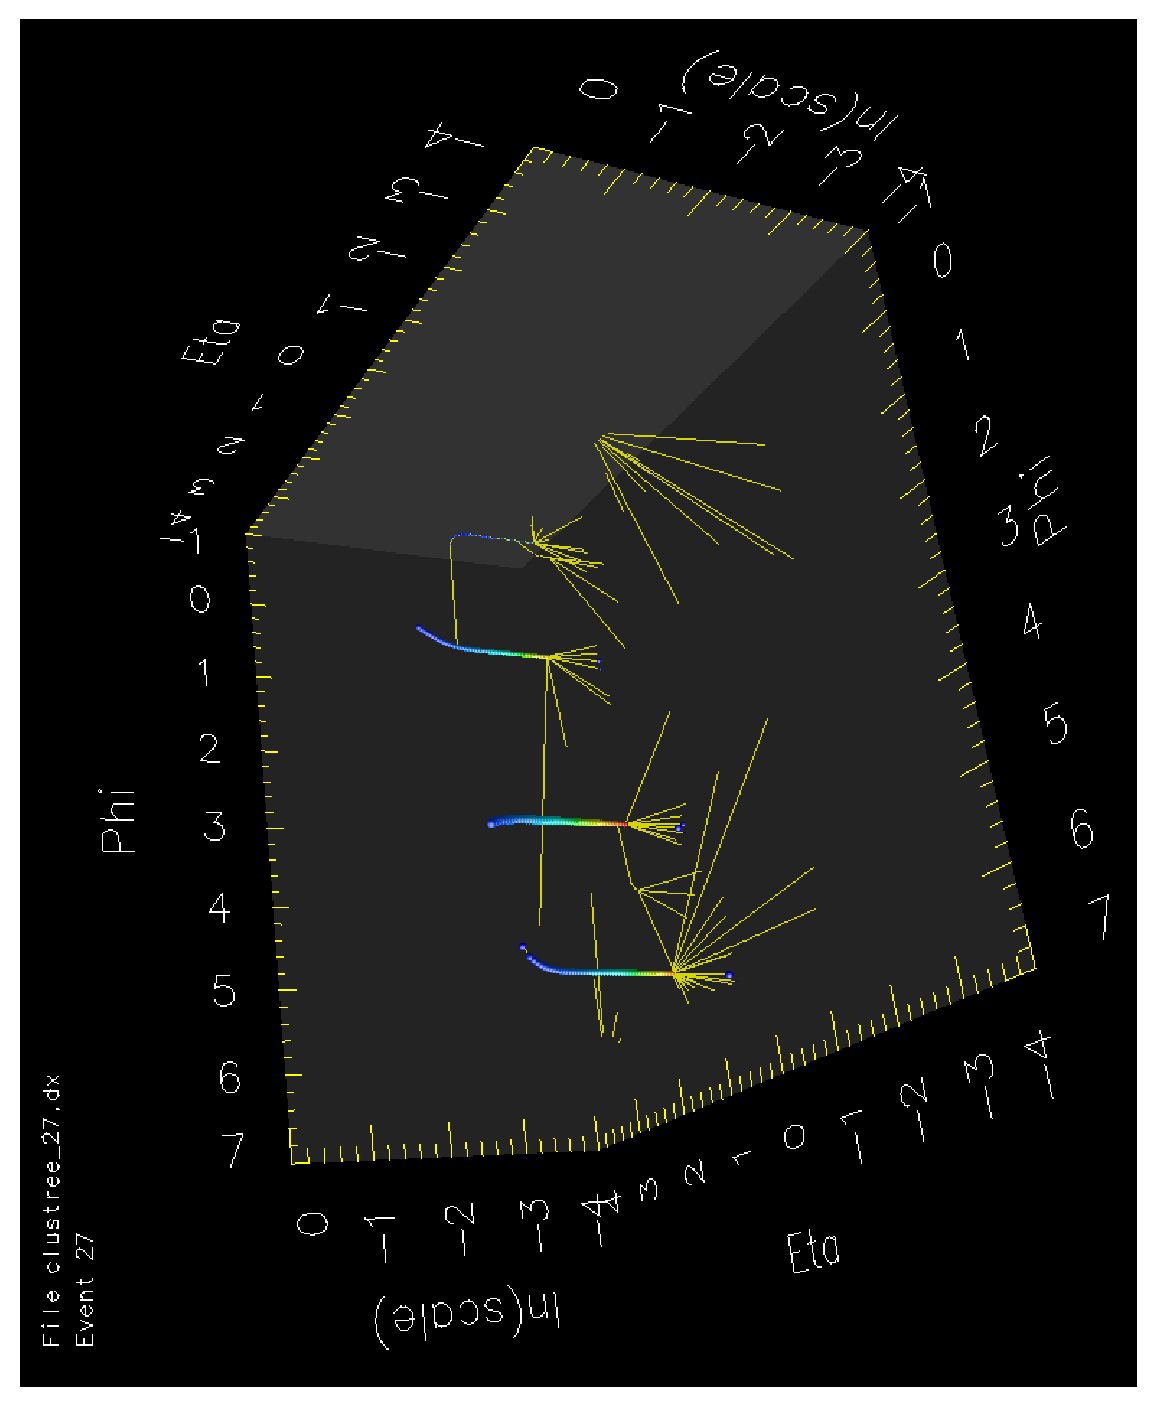
\epsfig{file=tree_image.eps,width=5.1in,angle=-90}
\caption{An example clustering tree image generated by OpenDX for
a four-jet event. Here, the quantity
$s^2 m(s)$, where $m(s)$ is the precluster magnitude, is mapped into
the glyph size and the scale-normalized Hessian
blob detector is mapped into the glyph color. The $\varphi$ variable
wraps around so that 0 and $2 \pi$ correspond to the same location. This is
why you see a bunch of connections apparently ending at $\varphi = 0$: they
actually ``tunnel'' from the right side of the image to the left and
continue towards the cluster near $\varphi = 2 \pi$.}
\label{opendxexample}
\end{center}
\end{figure}

Two OpenDX programs (or ``nets'') are provided with the FFTJet
package in the ``opendx'' subdirectory:  \verb[view_one_tree.net[ and
\verb[view_tree_sequence.net[. The first one can be used to visualize
a single clustering tree saved in a proper format. The second one
is intended for browsing through many trees which correspond to different
events, one file per event. The instructions for using these programs
can be found in the ``README'' file in the ``opendx'' subdirectory.

If the user wants to view the clustering trees using other types
of visualization software (or to just dump the information
to disk in a human-readable
form), we suggest implementing the visualization system
interface by deriving it from the
\cname{AbsTreeFormatter} abstract class.
Use of \cname{AbsTreeFormatter} will result in
a uniform interface for saving the tree data
independent from a particular visualization  system used.

\subsection{Persistent Interpolation Tables}
\label{sec:interptables}

The FFTJet package provides facilities for building detailed
jet models using multidimensional interpolation tables.
The jet energy profiles in the \epspace can be represented
using 3d tables (for example, with equidistant grids
in the $\eta$, $\varphi$, and $\log(s) \equiv \log(1/p_T)$ variables), and
detector-level fragmentation function can be represented
using 4d tables. Normally, construction of such tables
should proceed with the help of a convenient
histogramming and data visualization package.

In order to build a detector-level fragmentation function,
one has to simulate the detector response to a large
number of jets. It is important to use the same energy discretization
grid binning
as the one which will be later used for jet reconstruction
because binning effects become important for the narrow neutral
``core'' of the jet which deposits most of its energy in just
a few calorimeter towers. A typical HEP calorimeter has a few
thousands of towers, and 12 to 16 bit linearized ADC dynamic
range is not uncommon. This means that a complete, uncompressed 
fragmentation function implemented using a rectangular equidistant
grid in the $(\eta, \varphi, \varepsilon, \log(s))$ variables
could require, roughly, from 20 to 1000 MBytes of memory per
recombination scale. This clearly becomes a problem in case
one wants to use a reasonably large number of scales.

Fortunately, the detector-level fragmentation function becomes
very small very quickly away from the jet core. Only particles
with small energies can be radiated at large angles, and the
same is true for particle deviations due to the presence of
magnetic field. This, naturally, leads to the detector fragmentation
function representation in which, for each value of
$(\Delta \eta, \Delta \varphi)$ from the jet direction,
only the occupancy of the first few energy bins has
to be stored, and the occupancy for higher $\varepsilon$
values is 0. This representation is realized in the FFTJet
package by the \cname{InterpolatedMembershipFcn} class.

The user is supposed to construct an \cname{InterpolatedMembershipFcn}
object incrementally, by sequentially feeding it the data for each
recombination scale in the full equidistant
rectangular grid format (3d histograms).
The object will automatically determine
the energy range to use in the
compressed representation for each $(\eta, \varphi)$ bin.
Once the \cname{InterpolatedMembershipFcn} is fully constructed,
it can be saved to disk in a binary format using the ``write''
function. The memory saving factor which \cname{InterpolatedMembershipFcn}
achieves in comparison with a~``full'' 4d representation is
typically a few hundred.

Lower-dimensional interpolated functions can be stored in the binary format
as well (without compression): \cname{InterpolatedKernel3d} can
be used to model arbitrary scale-dependent jet energy profiles,
and \cname{InterpolatedKernel} can be used to represent
functions whose width in the \epspace changes in proportion to the scale
but the shape (skewness, kurtosis) remains constant.

In all cases, interpolations are performed linearly in the
$\eta$, $\varphi$, and $\varepsilon$ variables. Interpolation
in the scale variable is linear either in $s$ or in $\log(s)$. 
Interpolation in a~$q$-dimensional hyperrectangular grid is performed
using the $2^q$ points at the vertices of the hyperrectangular
cell inside which the point of interest is located. If the cell
is shifted and scaled in such a~way that it becomes a hypercube
with diagonal vertices at $(0, 0, ..., 0)$ and $(1, 1, ..., 1)$ then
the interpolation formula can be compactly written as
$$
f(x_1, x_2, ..., x_q) = \sum_{\substack{
m_1 = \,0, 1\\
m_2 = \,0, 1\\
...\\
m_q = \,0, 1\\
}}  f(m_1, m_2, ..., m_q) \prod_{k=1}^q x_k^{m_k} (1 - x_k)^{1 - m_k}
$$

At present time, the author of the FFTJet package has no access to a
big-endian computer, so a~platform-independent implementation of the
binary I/O interface for the interpolated functions
was not attempted. All binary data is currently
stored in the native format.
Note that the binary read/write
operations are not performed by various object
serialization methods directly. Instead, all of them proceed through
another layer of functions defined in the ``binaryIO.hh''
header.\footnote{These functions look somewhat like a templated
version of the XDR library and might actually use XDR in the future.}
If necessary, it will be easy to provide a~platform-independent
binary I/O interface by properly adapting these functions.

\subsection{Jet Energy Correction}

Inversion of the jet energy response curve is a common procedure
encountered in jet reconstruction, often termed ``jet energy correction''.
Typically, the response curve is defined as
the mean (peak, median, {\it etc}) ratio between the reconstructed jet
predictor quantity (jet $p_T$ or $E_T$) and the actual jet
(or parton) $p_T$ known from Monte Carlo. This ratio is initially
constructed as a function of the actual jet $p_T$ and, possibly,
some other parameters (in practice, $\eta$ of the {\it reconstructed} jet
is often used as the second parameter).

The simplest reasonable estimator of the actual jet $p_T$ can be obtained
from the reconstructed jet information
by applying the inverse jet energy response
function to the measured predictor quantity.\footnote{This estimator
is neither unbiased nor efficient. Estimation of the actual jet $p_T$
given the measured predictor is a stochastic inverse problem
complicated by censoring which occurs due to pattern
recognition inefficiency at low $p_T$ values.
Proper treatment of this
problem is beyond the scope of this note.} FFTJet
provides several classes and functions which facilitate
the task of inverting the response curve:
\begin{itemize}
\item \cname{invertJetResponse} (header file ``invertJetResponse.hh''). This
function solves the equation $x f(x) = y$ numerically 
for unknown $x$ under the following
assumptions: 

a) $f(x) > 0$ for every $x$, 

b) $y \ge 0$,

c) $x f(x)$ is monotonously increasing, and

d) $\lim_{x \rightarrow 0} (x f(x)) = 0$.

\item \cname{invertJetResponse2d} (header file ``invertJetResponse.hh'').
This function solves the same equation for a function which, in addition
to $x$, depends on another parameter which is assumed to be constant
during equation solving.

\item \cname{JetMagnitudeMapper} (header file ``JetMagnitudeMapper.hh'').
This class builds the inverse jet response curve numerically assuming
that the response function depends only on one variable ({\it e.g.,} jet $p_T$).

\item \cname{JetMagnitudeMapper2d} (header file ``JetMagnitudeMapper2d.hh'').
This class builds the inverse jet response curve numerically assuming
that the response function depends on two variables ({\it e.g.,} jet $p_T$
and the recombination scale at which jet energy was reconstructed).
\end{itemize}
\noindent In addition to the classes listed above, the classes
\cname{IdleJetCorrector} and \cname{InvalidJetCorrector} (header file ``AbsJetCorrector.hh'')
can sometimes be useful. The \cname{IdleJetCorrector} class does not perform
any correction, so it can be substituted instead of some other corrector when
the jet response curve is constructed (assuming that the application code
performs jet corrections via the interface provide by the
\cname{AbsJetCorrector} abstract base class).
\cname{InvalidJetCorrector}
can be used as a convenient and safe placeholder during code development.

The classes which represent
inverse jet response curves are not persistent. However,
their construction from the ``direct'' response curves usually takes
a negligible amount of CPU time since it has to be performed only once.
Arbitrary ``direct'' curves can be stored in binary format using
serializable classes \cname{LinearInterpolator1d} and
\cname{LinearInterpolator2d}.

\newpage
\appendix
% \addtocontents{toc}{\protect\contentsline{section}{Appendix:}{}}
\section{FFTJet Kernel Functions}
\label{appKern}

\subsection{2-d Kernels}

Most 2-d kernels provided by the FFTJet package can be
made axially symmetric by a~linear transformation in the \epspace\!\!.
All such kernels have the following functional form:
$$
K(\eta, \varphi, s) = \frac{1}{h_{\eta} h_{\varphi}} G(r^2), \ \ \mbox{where}\ r^2 = \left(\frac{\eta}{h_{\eta}}\right)^2 + \left(\frac{\varphi}{h_{\varphi}}\right)^2, \ h_{\eta} = b_{\eta} s^p, \ h_{\varphi} = b_{\varphi} s^p,
$$
$b_{\eta}$ and $b_{\varphi}$ are some positive constants and $p$ is an integer
(-1, 0, and 1 are the most meaningful values for the parameter $p$).
$G(r^2)$ functions are listed in Table~\ref{table:symkernels} together
with their corresponding class names and header files.
If you want to use an axially symmetric kernel not provided by the package,
it may be useful to derive your kernel class from \cname{AbsSymmetricKernel}
(see files ``Kernels.hh''
and ``Kernels.cc'' for examples of such classes). Then your kernel will automatically
handle bandwidth calculations in the manner just described.

\begin{table}[h!]
\caption{Axially symmetric 2-d kernels.
The normalization constant $N$, when not given explicitly,
is calculated so that
$\int_0^{\infty} G(r^2) 2 \pi r dr = 1$.}
\label{table:symkernels}
\begin{center}
\noindent\begin{tabular}{|c|c|c|} \hline
$G(r^2)$ & Class Name & FFTJet Header File \\ \hline\hline
$\begin{array}{ll}
  N (1 - r^2)^n, & r^2 < 1\\
  0, & r^2 \ge 1
\end{array}$ & \cname{SymmetricBeta} & Kernels.hh \\ \hline
$\begin{array}{ll}
  \frac{3}{\pi} (1 - \sqrt{r^2}), & r^2 < 1\\
  0, & r^2 \ge 1
\end{array}$ & \cname{Linear2d} & Kernels.hh \\ \hline
$\frac{1}{2 \pi} e^{-r^2/2}$ & \cname{Gauss2d} & Kernels.hh \\ \hline
$ N e^{-(r^2/2)^{\alpha/2}}$ & \cname{SubGauss} & Kernels.hh \\ \hline
$\begin{array}{ll}
  N e^{-r^2/2}, & \sqrt{r^2} \le a\\
  N e^{a \,(a/2-\sqrt{r^2})}, &  \sqrt{r^2} > a
\end{array}$ & \cname{Huber2d} & Kernels.hh \\ \hline
$\frac{N}{1 + r^{2n}}$ & \cname{InvPower2d} & Kernels.hh \\ \hline
$\begin{array}{cl}
  \mbox{Arbitrary (interpolated} &\\
  \mbox{from a table of values)}, & r^2 < 1\\
  0, & r^2 \ge 1
\end{array}$ & \cname{ProfileKernel} & ProfileKernel.hh \\ \hline
$\begin{array}{ll}
  \mbox{Arbitrary (interpolated} &\\
  \mbox{from a table of function} &\\
  \mbox{logarithm values)}, & \sqrt{r^2} \le a\\
  \ \ \ \ \ \ \ G(a^2) e^{-k (\sqrt{r^2} - a)}, &  \sqrt{r^2} > a
\end{array}$ & \cname{LogProfileKernel} & LogProfileKernel.hh \\ \hline
\end{tabular}
\end{center}
\end{table}

In addition to the kernels listed
in Table~\ref{table:symkernels}, the following
2-d kernel classes are provided:
\begin{itemize}
\item \cname{InterpolatedKernel} (header ``InterpolatedKernel.hh'').
This class implements an arbitrary kernel function without
axial symmetry whose
width in the \epspace changes with the scale
in a way specified below and whose shape (skewness, kurtosis, {\it etc})
remains constant. Such a kernel is described by the following functional form:
$$
K(\eta, \varphi, s) = \frac{1}{h_{\eta} h_{\varphi}} H(\frac{\eta}{h_{\eta}}, \frac{\varphi}{h_{\varphi}}), \ h_{\eta} = b_{\eta} s^p, \ h_{\varphi} = b_{\varphi} s^p.
$$
$b_{\eta}$ and $b_{\varphi}$ are some positive constants and $p$ is an integer.
$H(x, y)$ values are tabulated on a 2d equidistant rectangular grid. In between, the
function values are interpolated linearly. If you would like to implement
your own kernel which handles bandwidth scaling in the same manner, derive your
class from \cname{AbsScalableKernel}.

\item \cname{InterpolatedKernel3d} (header ``InterpolatedKernel3d.hh''). An
arbitrary kernel function whose values are linearly interpolated from
points on a 3d equidistant rectangular grid.

\item \cname{DiscreteGauss2d} (header ``DiscreteGauss2d.hh''). Gaussian
kernel corrected for the energy flow discretization effects. This kernel is,
essentially, the Green's function for the two-dimensional
anisotropic diffusion equation with
the discretized Laplacian operator.
Unlike the standard Gaussian kernel which 
no longer conforms to the scale space axioms
when its width becomes comparable to the grid bin size,
\cname{DiscreteGauss2d} remains compliant, and
gracefully converges to the {\it discrete} delta function
at the limit of zero scale. This kernel is defined by its
Fourier transform representation:
% \[
% \begin{array}{rcrl}
% \mbox{Re}(F(u, v)) & = & \exp \,\biggl\{(1 - \gamma) & \left[\frac{\sigma_{\eta}^2}{(\Delta \eta)^2} (\cos (u) -1) + \frac{\sigma_{\varphi}^2}{(\Delta \varphi)^2} (\cos (v) -1) \right] +\\
% & & \gamma & \left[  \left(\frac{\sigma_{\eta}^2}{(\Delta \eta)^2} + \frac{\sigma_{\varphi}^2}{(\Delta \varphi)^2}\right)    \frac{2 (\Delta \eta)^2 (\Delta \varphi)^2}{((\Delta \eta)^2 + (\Delta \varphi)^2)^2} \bigl(\cos (u) \cos (v) - 1\bigr) \ + \right.\\
% & & & \left.\frac{1}{4} \left(\frac{\sigma_{\eta}^2}{(\Delta \eta)^2} - \frac{\sigma_{\varphi}^2}{(\Delta \varphi)^2}\right) \bigl(\cos (u) - \cos (v)\bigr)\right] \biggr\}\\
% \mbox{Im}(F(u, v)) & = & 0,  \ \ \ \ \ \ \ \ \ \  \ \ \ \ \ &
% \end{array}
% \]
\[
\begin{array}{rcl}
\mbox{Re}(F(u, v)) & = & \exp \left(\frac{\sigma_{\eta}^2}{(\Delta \eta)^2} (\cos (u) -1) + \frac{\sigma_{\varphi}^2}{(\Delta \varphi)^2} (\cos (v) -1) \right), \\
\mbox{Im}(F(u, v)) & = & 0,
\end{array}
\]
where

$u = \frac{2 \pi k}{N_{\eta}}$, $k \in \{0, 1, ..., N_{\eta}-1\}\,$ is the $\eta$ frequency.

$v = \frac{2 \pi m}{N_{\varphi}}$, $m \in \{0, 1, ..., N_{\varphi}-1\}\,$  is the $\phi$ frequency.

$\Delta \eta = \frac{2 \pi}{N_{\eta}}$ is the {\it effective} width of the grid cells in $\eta$ (scaled so that the full $\eta$ range of the grid is $2 \pi$).

$\Delta \varphi = \frac{2 \pi}{N_{\varphi}}$ is the width of the grid cells in $\varphi$.

$\sigma_{\eta}$ is the {\it effective} kernel width parameter in $\eta$. In the
limit of small cell sizes and when $\sigma_{\eta} \ll 2 \pi$, it corresponds
to the standard deviation of the Gaussian kernel.

$\sigma_{\varphi}$ is the kernel width parameter in $\varphi$.

% $\gamma$ is the direction mixing parameter for the discretized Laplacian.
% $\gamma = 0$ means that the Laplacian is evaluated along the $\eta$ and
% $\varphi$ directions using the standard 5-point formula,
% $\gamma = 1$ means that the Laplacian
% is calculated along the grid diagonal, and values
% in between correspond to the mixture of the two. Reasonable values for
% this parameter are $0 \le \gamma \le 1/2$, while $\gamma = 1/3$
% results in the ``most isotropic'' calculation.

\noindent The rationale for this type of kernel
can be found in Ref.~\cite{ref:discretescalespace}.

\item \cname{DeltaFunctionKernel} (header ``Kernels.hh'').
Represents 2-d delta function $a \,\delta(\eta, \varphi)$.
The method ``double operator()(double eta, double phi, double s)'' of
the ``DeltaFunctionKernel'' class returns 0 when
either ``eta'' or ``phi'' argument is not equal to 0, and results
in a run-time error when both ``eta'' and ``phi'' are 0. Thus, using
``operator()'' of this and other kernels which involve delta functions
is not recommended in the application code. Instead,
use the ``rectangleAverage''
method which behaves as expected.

\item \cname{PythiaKernel\_30\_100\_v0} (header ``PythiaKernel\_30\_100\_v0.hh'').
Angular energy profile of the Pythia light quark
single jet gun in the absence
of magnetic field.
Accurate for jets with transverse momenta $p_{T} > 30$~GeV/$c$ or so. For such
jets, the width of the angular profile scales in the inverse proportion to jet $p_{T}$.
The scale parameter
for this kernel should be set to $1/(\mbox{jet}\ p_{T})$.

\item \cname{RealFrequencyKernel} (header ``RealFrequencyKernel.hh'').
Can be used to represent kernels whose Fourier transforms are pure real.
It takes any kernel in the \epspace and substitutes $\omega_{\eta}$,
$\omega_{\varphi}$ in place of $\eta$ and $\varphi$ in order to calculate
the real part of the transform. The imaginary part is set to 0.

\item \cname{PhiGauss} (header ``PhiKernels.hh''). A product of the delta
function in $\eta$ and the Gaussian density in $\varphi$:
$K(\eta, \varphi, s) = \frac{\delta(\eta)}{\sqrt{2 \pi} h_{\varphi}} e^{-\frac{\varphi^2}{2  h_{\varphi}^2}}$, $h_{\varphi} = b_{\phi} s^p$, where $b_{\varphi}$ is some
positive constant and $p$ is an integer.

\item \cname{PhiProfileKernel} (header ``PhiKernels.hh'').
 A product of the delta function in $\eta$ and an arbitrary even
function of $\varphi$:
$K(\eta, \varphi, s) = \frac{\delta(\eta)}{h_{\varphi}} P(\varphi/h_{\varphi})$,
$h_{\varphi} = b_{\phi} s^p$, where $b_{\varphi}$ is some
positive constant and $p$ is an integer. The function $P(\varphi)$
is represented by a table of its values on the equidistant
grid which covers the interval $[0, \pi/2]$. It is assumed that $P(\varphi) = 0$
when $\varphi \ge \pi/2$, and that $P(-\varphi) = P(\varphi)$.

\item \cname{CompositeKernel} (header ``CompositeKernel.hh'').
Can be used to calculate
a linear combination of kernels: $\sum_{i} a_i K_i(\eta, \varphi, s)$,
where $a_i$ are fixed constants.

\item \cname{MagneticSmearingKernel} (header ``MagneticSmearingKernel.hh'').
This kernel can be used to model the angular smearing of a jet due to the
presence of a magnetic field in the detector. It is assumed that the magnetic
field is directed along the beam axis.

\end{itemize}

\subsection{1-d Kernels}

The 1-d kernels provided by the FFTJet package are intended for use
with the \cname{SequentialConvolver} and \cname{FrequencySequentialConvolver}
classes. The following functions are implemented:

\begin{itemize}
\item \cname{Gauss1d} (header ``Kernels1d.hh''). This kernel looks like
$$
K(x, s) = \frac{1}{b s^p} G \left( \frac{x}{b s^p} \right), \ \ G(y) = \frac{1}{\sqrt{2 \pi}} e^{-\frac{y^2}{2}}
$$
where $b$ is some positive constants and $p$ is an integer. The
scaling behavior which relates $K(x, s)$ and $G(y)$ is built into the
\cname{AbsScalableKernel1d} base class from which \cname{Gauss1d}
is derived. If you need to implement your own 1-d kernel with
similar scaling behavior, derive it from \cname{AbsScalableKernel1d}.

\item \cname{SymmetricBeta1d} (header ``Kernels1d.hh'').
This class is also derived from \cname{AbsScalableKernel1d} using
$$
G(y) = \left\{ \begin{array}{ll} 
               N (1 - y^2)^n, & y^2 < 1 \\
               0,             & y^2 \ge 1
               \end{array}
         \right.
$$
where the normalization constant $N$ is calculated so
that $\int_{-1}^{1}G(y) dy = 1$.

\item \cname{DeltaFunction1d} (header ``Kernels1d.hh'').
This kernel represents the 1-d delta function $a \,\delta(x)$.
Evaluation of this function at $x = 0$ will result in a run-time error.
Use ``intervalAverage'' method instead.

\item \cname{DiscreteGauss1d} (header ``DiscreteGauss1d.hh'').
This is a 1-d version of \cname{DiscreteGauss2d}. The kernel
is defined by its Fourier transform:
\[
\begin{array}{rcl}
\mbox{Re}(F(u)) & = & \exp \left(\frac{\sigma^2}{\Delta^2} (\cos (u) -1)\right), \\
\mbox{Im}(F(u)) & = & 0,
\end{array}
\]
where

$u = \frac{2 \pi k}{N}$, $k \in \{0, 1, ..., N-1\}\,$ is the Fourier frequency.

$\Delta = \frac{2 \pi}{N}$ is the effective width of the grid cells.

$\sigma$ is the effective kernel width parameter.

\item \cname{RealFrequencyKernel1d} (header ``RealFrequencyKernel1d.hh'').
Can be used to represent kernels whose Fourier transforms are pure real
and can be calculated with any other 1-d kernel. The imaginary part
of the transform is set to 0.
\end{itemize}

Classes \cname{DefaultKernel1dFactory} and \cname{DefaultKernel2dFactory} 
(header files ``Kernel1dFactory.hh'' and ``Kernel2dFactory.hh'', respectively)
can be utilized to simplify creation
of kernel objects in various interpretive language data analysis environments.

\newpage
\addcontentsline{toc}{section}{References}
\begin{thebibliography}{99}

\bibitem{ref:cheng} {
Y. Cheng, ``Mean Shift, Mode Seeking, and Clustering'', IEEE Trans. Pattern
Analysis and Machine Intelligence, Vol 17, pp. 790-799, 1995.}

\bibitem{ref:modetree} {
M.C. Minnotte and D.W. Scott, ``The Mode Tree: a Tool for
Visualization of Nonparametric Density Features'', 
J. Comp. Graph. Statist., Vol 2, pp. 51-68, 1993.}

\bibitem{ref:igv2006} {
I. Volobouev, ``Density-Based Clustering and Jet Reconstruction'',
presentation at the MC4LHC Workshop, CERN, July 2006.}

\bibitem{ref:kde} {
D.W.~Scott, ``Multivariate Density Estimation: Theory, Practice, and
Visualization'', Wiley, 1992.}

\bibitem{ref:clhep} {
http://www.cern.ch/clhep
}

\bibitem{ref:numrecipes} {
W.H.~Press, S.A.~Teukolsky, W.T.~Vetterling, and B.P.~Flannery,
``Numerical Recipes: the Art of Scientific Computing'', 3rd ed.,
Cambridge University Press, 2007.
}

\bibitem{ref:balltree} {
 S. M. Omohundro, ``Five Balltree Construction Algorithms'',
ICSI Technical Report TR-89-063, 1989.
}

\bibitem{ref:dendrogram} {
http://en.wikipedia.org/wiki/Dendrogram
}

\bibitem{ref:blobdetect} {
http://en.wikipedia.org/wiki/Blob\_detection

The utility of the standard scale-normalized Laplacian and Hessian-based
blob detectors in the Gaussian
scale space is not clear and deserves further study.
The main problem here is that jets do not have
a well-defined radial extent in the \epspace\!\!.
The average angular jet energy profile, $E(r)$,
where $r = \sqrt{\eta^2 + \varphi^2}$,
behaves approximately as $r^{-3}$ for large values of $r$
(according to Pythia). If such a behavior is extrapolated
to infinity then the second moment integral
$\int{r^2 E(r) 2 \pi r dr}$ diverges.
(Here, $E_{jet} = \int{E(r) 2 \pi r dr}$.)}

\bibitem{ref:opendx}
http://www.opendx.org/

\bibitem{ref:discretescalespace} {
T. Lindeberg, ``Scale-Space for Discrete Signals'',
IEEE Trans. Pattern Analysis and Machine Intelligence,
Vol 12, pp. 234-254, 1990.}

\end{thebibliography} 

\newpage
\addcontentsline{toc}{section}{Functions and Classes}
\printindex

\end{document}
